%%%%%%%%%%%%%%%%%%%%%%%%%%%%%%%%%%%%%%%%%%%%%%%%%%%%%%%%%%%%%%%%%%%%%%%%

%%% LaTeX Template for AAMAS-2025 (based on sample-sigconf.tex)
%%% Prepared by the AAMAS-2025 Program Chairs based on the version from AAMAS-2025. 

%%%%%%%%%%%%%%%%%%%%%%%%%%%%%%%%%%%%%%%%%%%%%%%%%%%%%%%%%%%%%%%%%%%%%%%%

%%% Start your document with the \documentclass command.


%%% == IMPORTANT ==
%%% Use the first variant below for the final paper (including auithor information).
%%% Use the second variant below to anonymize your submission (no authoir information shown).
%%% For further information on anonymity and double-blind reviewing, 
%%% please consult the call for paper information
%%% https://aamas2025.org/index.php/conference/calls/submission-instructions-main-technical-track/

%%%% For anonymized submission, use this
\documentclass[sigconf,anonymous]{aamas} 

%%%% For camera-ready, use this
%\documentclass[sigconf]{aamas}

\usepackage{listings}
% \usepackage{xcolor}

\definecolor{codegreen}{rgb}{0,0.6,0}
\definecolor{codegray}{rgb}{0.5,0.5,0.5}
\definecolor{codepurple}{rgb}{0.58,0,0.82}
\definecolor{backcolour}{rgb}{0.95,0.95,0.92}
 
\lstdefinestyle{mystyle}{
    backgroundcolor=\color{backcolour},   
    commentstyle=\color{codegreen},
    keywordstyle=\color{magenta},
    numberstyle=\tiny\color{codegray},
    stringstyle=\color{codepurple},
    basicstyle=\footnotesize,
    breakatwhitespace=false,         
    breaklines=true,                 
    captionpos=b,                    
    keepspaces=true,                 
    numbers=left,                    
    numbersep=5pt,                  
    showspaces=false,                
    showstringspaces=false,
    showtabs=false,                  
    tabsize=2
}
 
\lstset{style=mystyle}

% --- Tickz
\usepackage{physics}
\usepackage{tikz}
\usepackage{amsmath}
\usepackage{mathdots}
% \usepackage{yhmath}
\usepackage{cancel}
\usepackage{color}
\usepackage{siunitx}
\usepackage{array}
\usepackage{cuted}
\usepackage{multirow}
% \usepackage{amssymb}
\usepackage{gensymb}
\usepackage{tabularx}
\usepackage{extarrows}
\usepackage{booktabs}
\usetikzlibrary{fadings}
\usetikzlibrary{patterns}
\usetikzlibrary{shadows.blur}
\usetikzlibrary{shapes}

% ---------

\usepackage{balance} % for balancing columns on the final page
\usepackage{csquotes}
% \usepackage{cite}
\newcommand{\probP}{I\kern-0.15em P}
\usepackage{etoolbox}
\patchcmd{\thebibliography}{\section*{\refname}}{}{}{}
% \usepackage{amsthm,amssymb,amsfonts}

\usepackage[T1]{fontenc}
\usepackage{graphicx}
\usepackage{hyperref}
\usepackage{color}
% \renewcommand\UrlFont{\color{blue}\rmfamily}

\usepackage[inline, shortlabels]{enumitem}
\usepackage{tabularx}
\usepackage{caption}
\usepackage{listings}
\usepackage{titlesec}
\usepackage{ragged2e}
% \usepackage[hyphens]{url}
\usepackage[linesnumbered,ruled,vlined]{algorithm2e}
\usepackage{float}

\usepackage[english]{babel}
\addto\extrasenglish{  
    \def\figureautorefname{Figure}
    \def\tableautorefname{Table}
    \def\algorithmautorefname{Algorithm}
    \def\sectionautorefname{Section}
    \def\subsectionautorefname{Subsection}
    \def\proofoutlineautorefname{Proof Outline}
}

\DeclareMathAlphabet\mathbfcal{OMS}{cmsy}{b}{n}

\newcommand{\supertiny}{\fontsize{1}{2}\selectfont}


%%%%%%%%%%%%%%%%%%%%%%%%%%%%%%%%%%%%%%%%%%%%%%%%%%%%%%%%%%%%%%%%%%%%%%%%

%%% AAMAS-2025 copyright block (do not change!)

\setcopyright{ifaamas}
\acmConference[AAMAS '25]{Proc.\@ of the 24th International Conference
on Autonomous Agents and Multiagent Systems (AAMAS 2025)}{May 19 -- 23, 2025}
{Detroit, Michigan, USA}{A.~El~Fallah~Seghrouchni, Y.~Vorobeychik, S.~Das, A.~Nowe (eds.)}
\copyrightyear{2025}
\acmYear{2025}
\acmDOI{}
\acmPrice{}
\acmISBN{}


%%%%%%%%%%%%%%%%%%%%%%%%%%%%%%%%%%%%%%%%%%%%%%%%%%%%%%%%%%%%%%%%%%%%%%%%

%%% == IMPORTANT ==
%%% Use this command to specify your EasyChair submission number.
%%% In anonymous mode, it will be printed on the first page.

\acmSubmissionID{<<EasyChair submission id>>}

%%% Use this command to specify the title of your paper.

\title[AAMAS-2025 CybMASDE]{A Method for Assisting Multi-Agent System Design Using Reinforcement Learning}

%%% Provide names, affiliations, and email addresses for all authors.

\author{Julien Soulé}
\affiliation{
  \institution{Univ. Grenoble Alpes}
  \city{Valence}
  \country{France}}
\email{julien.soule@lcis.grenoble-inp.fr}

\author{Jean-Paul Jamont}
\affiliation{
  \institution{Univ. Grenoble Alpes}
  \city{Valence}
  \country{France}}
\email{jean-paul.jamont@lcis.grenoble-inp.fr}

\author{Michel Occello}
\affiliation{
  \institution{Univ. Grenoble Alpes}
  \city{Valence}
  \country{France}}
\email{michel.occello@lcis.grenoble-inp.fr}

\author{Louis-Marie Traonouez}
\affiliation{
  \institution{Thales Land and Air Systems, BU IAS}
  \city{Rennes}
  \country{France}}
\email{louis-marie.traonouez@thalesgroup.com}

\author{Paul Théron}
\affiliation{
  \institution{AICA IWG}
  \city{La Guillermie}
  \country{France}}
\email{paul.theron@orange.fr}

\begin{abstract}
    Agent-Oriented Software Engineering (AOSE) methods typically rely on the designer's expertise to guide the development of a multi-agent system (MAS) that meets specific objectives within a given environment. Recent advancements in Multi-Agent Reinforcement Learning (MARL) suggest a more automated approach to exploring the design space. We introduce the SAMMASD (Semi-Automated MARL-based MAS Design) method, which integrates organizational specifications into MARL for MAS design and deployment. This method consists of four phases. The first phase models the real-world environment, objectives, and additional constraints—such as operational requirements—into a simulation. The second phase leverages multiple MARL algorithms to learn stable policies that achieve these objectives within the defined constraints. The third phase conducts a behavior analysis to infer emergent roles and objectives and to generate detailed "blueprints" for implementation. Finally, the development phase enables the automatic deployment of these policies in real-world environments, following validation in an emulated setting. We demonstrate SAMMASD in a warehouse flow management scenario involving robot agents, illustrating how the method can produce efficient and reliable MAS designs that streamline the design process.
\end{abstract}



%%% The code below was generated by the tool at http://dl.acm.org/ccs.cfm.
%%% Please replace this example with code appropriate for your own paper.


%%% Use this command to specify a few keywords describing your work.
%%% Keywords should be separated by commas.

\keywords{Agent-Oriented Software Engineering \and Multi-Agent Reinforcement Learning \and Assisted-Design \and Organizational Models}

%%%%%%%%%%%%%%%%%%%%%%%%%%%%%%%%%%%%%%%%%%%%%%%%%%%%%%%%%%%%%%%%%%%%%%%%

%%% Include any author-defined commands here.
         
% \newcommand{\BibTeX}{\rm B\kern-.05em{\sc i\kern-.025em b}\kern-.08em\TeX}

%%%%%%%%%%%%%%%%%%%%%%%%%%%%%%%%%%%%%%%%%%%%%%%%%%%%%%%%%%%%%%%%%%%%%%%%

\begin{document}

%%% The following commands remove the headers in your paper. For final 
%%% papers, these will be inserted during the pagination process.

\pagestyle{fancy}
\fancyhead{}

%%% The next command prints the information defined in the preamble.

\maketitle

%%%%%%%%%%%%%%%%%%%%%%%%%%%%%%%%%%%%%%%%%%%%%%%%%%%%%%%%%%%%%%%%%%%%%%%%

\section{Introduction}

Les systèmes multi-agents (SMA) sont au cœur de nombreuses applications, allant de la gestion d'entrepôts automatisés à la cybersécurité. Ces systèmes doivent permettre à plusieurs agents autonomes d'agir de manière coordonnée afin d'atteindre des objectifs communs dans des environnements complexes et dynamiques. Cependant, la conception de tels systèmes présente des défis majeurs en termes de robustesse, de sûreté et d'explicabilité des comportements des agents.

Les méthodes actuelles d'apprentissage par renforcement multi-agent (MARL) ont montré leur efficacité pour générer des politiques optimales dans des environnements dynamiques. Toutefois, ces approches manquent souvent de mécanismes explicites pour imposer des contraintes organisationnelles et garantir que les agents respectent des normes de sûreté essentielles pour des environnements critiques, comme la logistique en entrepôts ou la défense cybernétique.

Cet article présente une nouvelle méthode, \textbf{SAMMASD} (Semi-Automated MARL-based MAS Design), qui combine le framework \textbf{MOISE+MARL} avec la méthode d'évaluation \textbf{HEMM} pour inférer et appliquer des structures organisationnelles aux politiques apprises par les agents. L'intégration de \textbf{$mathcal{M}OISE^+$}, un modèle organisationnel orienté multi-agents, permet de contraindre l'apprentissage des agents en définissant des rôles et des missions, ce qui favorise l'émergence de comportements interprétables et conformes aux exigences de sûreté.

Le reste de cet article est structuré comme suit : la \autoref{sec:related_works} présente les travaux connexes dans le domaine du MARL et des modèles organisationnels pour SMA. La \autoref{sec:apprragh} décrit en détail les quatre phases de la méthode SAMMASD. Ensuite, la \autoref{sec:evaluation} discute des résultats expérimentaux obtenus dans un scénario de gestion de flux d'entrepôt. Enfin, la \autoref{sec:conclusion} conclut et propose des pistes de travail futures.

\section{Travaux connexes}
\label{sec:related_works}
La conception de systèmes multi-agents (SMA) assistée par des modèles organisationnels a été largement étudiée dans la littérature. En particulier, le modèle \textbf{$mathcal{M}OISE^+$}, introduit par Gleizes et al. \cite{gleize2008moise}, propose une structure formelle pour spécifier les rôles, les missions, et les relations entre agents dans un SMA. Ces spécifications permettent de guider le développement de systèmes complexes en assurant une cohérence entre les objectifs collectifs et les comportements individuels des agents. Cependant, $mathcal{M}OISE^+$ ne fournit pas de mécanismes pour intégrer directement l'apprentissage des politiques par renforcement, une lacune que notre travail cherche à combler.

D'un autre côté, les méthodes d'apprentissage par renforcement multi-agent (\textbf{MARL}) ont connu un essor ces dernières années, avec des approches telles que \textbf{MADDPG} (Multi-Agent Deep Deterministic Policy Gradient) \cite{lowe2017multi} et \textbf{Q-Mix} \cite{rashid2018qmix}. Ces algorithmes permettent aux agents d'apprendre des politiques optimales en collaboration ou en compétition dans des environnements partiellement observables. Néanmoins, ces méthodes se concentrent principalement sur la performance des politiques sans se soucier des contraintes organisationnelles ou des besoins en explicabilité, ce qui limite leur applicabilité dans des contextes nécessitant une coordination stricte entre agents.

Des travaux récents ont exploré des méthodologies agiles pour le développement de SMA, en combinant des approches orientées agent avec des pratiques agiles \cite{winikoff2021agile}. Ces méthodes visent à faciliter l'itération rapide dans la conception de SMA, mais elles n'intègrent pas directement les dynamiques d'apprentissage en MARL. Notre approche s'inscrit dans cette lignée en combinant l'apprentissage automatisé via MARL avec des spécifications organisationnelles, comblant ainsi le fossé entre les processus d'apprentissage et les exigences de conception organisationnelle.

\section{Approche de conception organisationnelle proposée pour les SMA}
\label{sec:apprragh}

Le coeur de la méthode SAMMASD est de considerer la conception d'un SMA comme un problème d'optimisation sous contraintes. La variable à optimiser est alors la \textbf{politique conjointe} qui est l'ensemble des logiques internes des agents leur permettant de déterminer leurs prochaines actions. L'objectif est de maximiser est la récompense cumulée en suivant cette politique conjointe sous des contraintes additionnelles données. SAMMASD inclue des spécifications organisationnelle en MARL comme contraintes additionnelles permettant à l'utilisateur de controler au moins partiellement non-seulement des comportements individuels des agents, mais aussi de pouvoir gérer l'ensemble des agents en ne jouant que sur celles-ci. Nous formalisons cette approche en proposant le framework MOISE+MARL. Puis, nous l'utilisons pour construire les quatre phases de notre méthode.

\subsection{\textbf{Framework MOISE+MARL}}

L'objectif est alors de guider l'apprentissage des agents en respectant des contraintes organisationnelles sous la forme de role et d'objectifs, tout en garantissant une efficacité suffisante des politiques apprises dans leur environment.
Nous formalisons cette idée en proposant le framework MOISE+MARL qui combine le formalisme d'un Decentralized Partially Observable Markov Decision Process (Dec-POMDP) avec le modèle organisationnel $\mathcal{M}OISE^+$.

\textbf{Dec-POMDP} \quad défini par un tuple $D = \langle N, S, A, P, R, \Omega, O, \gamma \rangle$, où :
%
\begin{itemize*}[label={},itemjoin={; }]
    \item $\mathcal{A}$, l'ensemble des $N \in \mathbb{N}$ agents
    \item $S$, l'ensemble des états possibles de l'environment (agents compris)
    \item $A = \times_{i=1}^N A_i $, l'ensemble des actions possibles pour chaque agent $i$
    \item $T: S \times A^N \to S$, la fonction de transition d'états qui définit le prochain état $s'$ à partir d'un état $s$ sous l'action conjointe $a$
    \item $R: S \times A^N \times  S \to \mathbb{R}$, la fonction de récompense associant une récompense $r$ à chaque transition $(s, a, s')$
    \item $\Omega = \times_{i=1}^N \Omega_i $ est l'ensemble des observations possibles pour chaque agent $i$
    \item $O: S \times A \to \Omega$ est la fonction d'observation qui définit la prochaine observation $\omega$ d'un agent lorsque ce dernier applique une action $a$ dans l'état $s$
    \item $\gamma \in [0, 1] $ est le facteur d'actualisation.
\end{itemize*}

$\mathbf{\mathcal{M}OISE^+}$ \quad défini par un tuple $\mathcal{OS} = \langle \mathcal{SS}, \mathcal{FS}, \mathcal{DS} \rangle$. Ici, nous présentons une version minimale du formalisme de $\mathcal{M}OISE^+$ :
\begin{itemize*}[label={},itemjoin={; }]
    \item $\mathcal{SS} = \langle \mathcal{R} \rangle$, les spécifications structurelles sont définies par un ensemble de rôles $\mathcal{R}$
    \item $\mathcal{FS} = \langle \mathcal{G}, \mathcal{M}, mo \rangle$, les spécifications fonctionnelles sont un ensemble d'objectifs $\mathcal{G}$, un ensemble de mission $\mathcal{M}$ et une fonction $mo: \mathcal{M} \to \mathcal{P}(\mathcal{G} \times [0,1])$ qui associe une mission $m \in \mathcal{M}$ à un ensemble d'objectifs chacun pondéré par un poids $\{(g_1,w_0), (g_2,w_1)\dots\}, w_i \in [0,1], g_i \in \mathcal{G}$
    \item $\mathcal{DS} = \mathcal{R} \times \mathcal{M} \times T_c \times \{0,1\}$, les spécifications déontiques comme un ensemble de 4-uplets $(\rho_a, m, \allowbreak t_c, p)$, signifiant respectivement qu'un agent jouant le rôle $\rho_a \in \mathcal{R}$ est autorisé (si $p = 0$) ou obligé (si $p = 1$) à s'engager dans la mission $m \in \mathcal{M}, \ m \subseteq \mathcal{G}$ pour une contrainte temporelle donnée $t_c \in \mathcal{TC}, t_c = \mathcal{P}(N)$ spécifiant une période pendant laquelle la permission/obligation est valide.
\end{itemize*}

Les \textbf{Constraint Guides} \quad sont trois nouvelles relations introduites pour décrire la logique des rôles et objectifs $\mathcal{M}OISE^+$ dans le formalisme Dec-POMDP:

\begin{itemize}
    \item \textbf{Role Action Guide} (RAG) \quad $rag: H \times \Omega \rightarrow \mathcal{P}(A \times \mathbb{R})$, la relation qui permet de modéliser un rôle comme un ensemble de règles qui à chaque couple constitué d'un historique $h \in H$ et d'une observation reçue par l'agent $\omega \in \Omega$, associe des actions attendues $A \in \mathcal{P}(A)$ chacune associée à une dureté de contrainte $ch \in [0,1]$ ($ch = 1$ par défaut). En restreignant le choix de la prochaine action parmi celles autorisées, l'agent est forcé d'adherer au comportement attendu du rôle
    \item \textbf{Role Reward Guide} (RRG) \quad $rrg: H \times \Omega \times A \to \mathbb{R} = \{r_m \text{ if } a \notin A_\omega \text{, } rag(h, \omega) = A_\omega \times \mathbb{R} \text{, } h \in H; \text{ else } 0\}$, la relation qui permet de modéliser un rôle en ajoutant un malus $r_m$ à la récompense globale si la dernière action choisie par l'agent $a \in A$ n'est pas autorisée. Cela vise à inciter l'agent à adherer au comportement attendu d'un role
    \item \textbf{Goal Reward Guide} (GRG) \quad $grg: H \rightarrow \mathbb{R}$, la relation qui permet de modéliser un objectif comme une contrainte molle en ajoutant un bonus $r_b \in \mathbb{R}$ à la récompense globale si l'historique de l'agent $h \in H$ contient une sous-séquence $h_g \in H_g$ caractéristique de l'objectif de sorte à inciter l'agent à trouver un moyen pour l'atteindre.
\end{itemize}

Enfin, pour lier les spécifications organisationnelles de $\mathcal{M}OISE^+$ aux "Constraint Guides" et aux agents, nous introduisons les relations \textbf{Linkers} suivantes :
\begin{itemize}
    \item \textbf{Agent to Role} (AR) \quad $ar: \mathcal{A} \to \mathcal{R}$, la relation bijective qui relie un agent à un rôle ;
    \item \textbf{Role to Constraint Guide} (RCG) \quad $rcg: \mathcal{R} \rightarrow rag \cup rrg$, la relation qui associe chaque rôle de $\mathcal{M}OISE^+$ à une relation $rag$ ou $rrg$, forçant/incitant l'agent à suivre les actions attendu pour le role $\rho \in \mathcal{R}$ ;
    \item \textbf{Goal to Constraint Guide} (GCG) \quad $gcg: \mathcal{G} \rightarrow grg$ la relation qui lie les objectifs aux relations de trf, en représentant les objectifs sous forme de récompenses dans le MARL.
\end{itemize}

MOISE+MARL est donc défini par le tuple $MM = \langle D, \mathcal{OS}, ar, rcg, \allowbreak gcg, rag, rrg, grg\rangle$.
Résoudre le problème décrit par MOISE+MARL implique de trouver une politique conjointe $\pi^{j} = \Omega^{N} \to A^{N} = \{\pi^j_0,\pi^j_1\dots\pi^j_N\}$ qui maximise la fonction de valeur $V^{\pi^{j}}$ (ou atteint un seuil minimal) qui représente la récompense cumulative espérée en partant d'un état initial $s \in S$ et en suivant la politique conjointe $\pi^{j}$, en appliquant succesivement les actions conjointes $a^{j} \in A^N$ sous les contraintes additonnelles des "Constraint Guides" (en incluant les "Linkers"). Les agents parcourent alors chacun une trajectoire (aussi appelée historique) $h \in H, h = \langle(o_0,a_0), (o_1,a_1)\dots\rangle$. La fonction de valeur à maximiser (ou atteindre un seuil minimal) est décrite dans le cas où les agents agissent les uns après les autres séquentiellement (mode Agent Environnement Cycle - AEC) dans la \hyperref[eq:single_value_function]{Definition 1} en adaptant sa définition pour les rôles (en rouge) et les missions (en bleu), impactant ainsi l'espace des actions et la récompense. La figure \autoref{fig:mm_synthesis} illustre synthetiquement les liens ente $\mathcal{M}OISE^+$ et Dec-POMDP au travers du framework MOISE+MARL.

\begin{figure*}[h!]
  \centering
  


\tikzset{every picture/.style={line width=0.75pt}} %set default line width to 0.75pt        

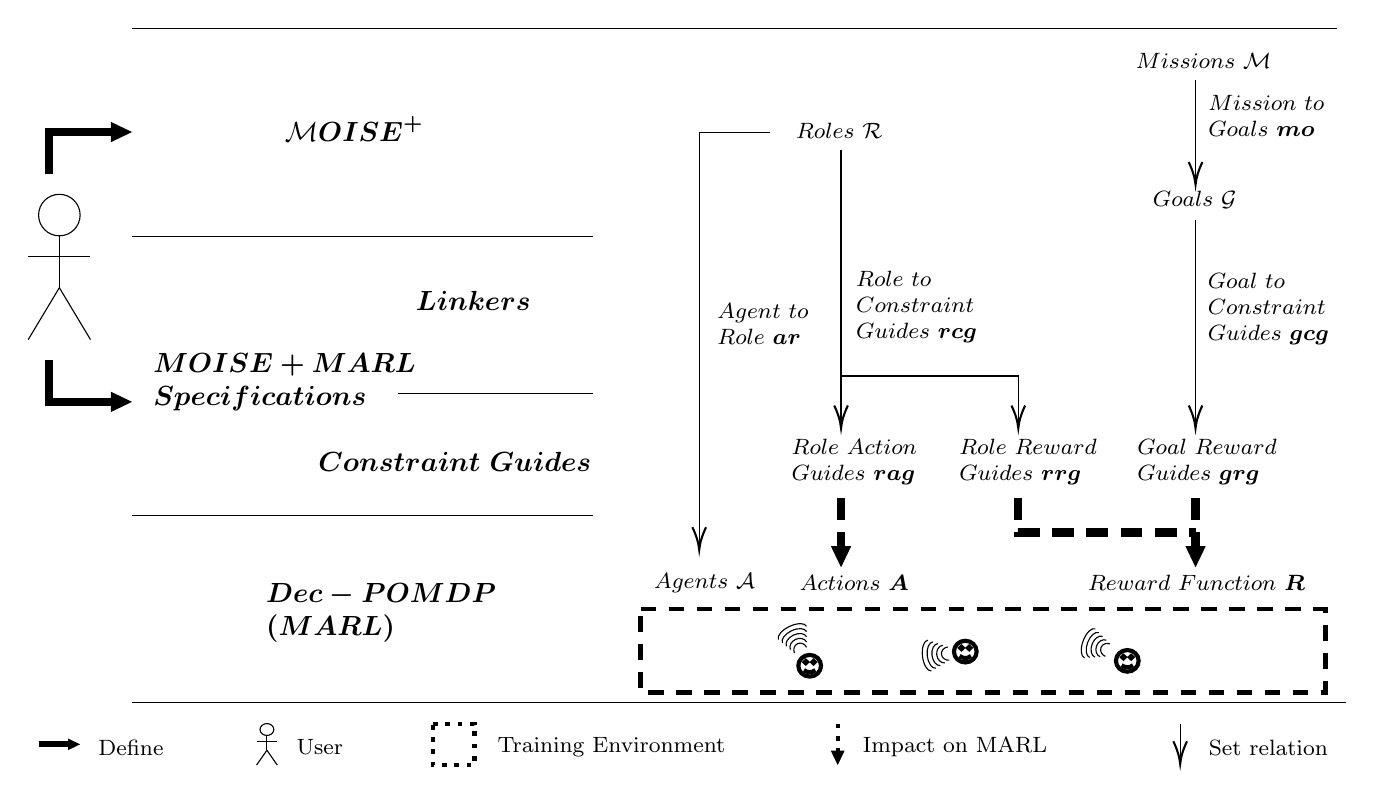
\begin{tikzpicture}[x=0.75pt,y=0.75pt,yscale=-1,xscale=1]
%uncomment if require: \path (0,2584); %set diagram left start at 0, and has height of 2584

%Straight Lines [id:da43492967264827187] 
\draw    (60,2000.54) -- (282.04,2000.54) ;
%Straight Lines [id:da5909021483617971] 
\draw    (572.41,1925.14) -- (572.41,1973.4) ;
\draw [shift={(572.41,1975.4)}, rotate = 270] [color={rgb, 255:red, 0; green, 0; blue, 0 }  ][line width=0.75]    (10.93,-3.29) .. controls (6.95,-1.4) and (3.31,-0.3) .. (0,0) .. controls (3.31,0.3) and (6.95,1.4) .. (10.93,3.29)   ;
%Straight Lines [id:da21005556631392852] 
\draw    (60,2134.58) -- (282.04,2134.58) ;
%Straight Lines [id:da3719427574917362] 
\draw    (188,2076) -- (282,2076) ;
%Straight Lines [id:da9250384002206431] 
\draw    (60,2225) -- (129,2225) -- (143,2225) -- (645,2225) ;
%Straight Lines [id:da8740103748997392] 
\draw    (60,1900.01) -- (640.73,1900.01) ;
%Straight Lines [id:da7641738582470461] 
\draw    (367.45,1950.27) -- (333.28,1950.27) -- (333.28,2149.33) ;
\draw [shift={(333.28,2151.33)}, rotate = 270] [color={rgb, 255:red, 0; green, 0; blue, 0 }  ][line width=0.75]    (10.93,-3.29) .. controls (6.95,-1.4) and (3.31,-0.3) .. (0,0) .. controls (3.31,0.3) and (6.95,1.4) .. (10.93,3.29)   ;
%Straight Lines [id:da17224242539642898] 
\draw    (401.61,1958.65) -- (401.61,2067.56) -- (401.61,2067.56) -- (401.61,2090.69) ;
\draw [shift={(401.61,2092.69)}, rotate = 270] [color={rgb, 255:red, 0; green, 0; blue, 0 }  ][line width=0.75]    (10.93,-3.29) .. controls (6.95,-1.4) and (3.31,-0.3) .. (0,0) .. controls (3.31,0.3) and (6.95,1.4) .. (10.93,3.29)   ;
%Straight Lines [id:da195049508631697] 
\draw    (401.61,2067.56) -- (487.01,2067.56) -- (487.01,2090.69) ;
\draw [shift={(487.01,2092.69)}, rotate = 270] [color={rgb, 255:red, 0; green, 0; blue, 0 }  ][line width=0.75]    (10.93,-3.29) .. controls (6.95,-1.4) and (3.31,-0.3) .. (0,0) .. controls (3.31,0.3) and (6.95,1.4) .. (10.93,3.29)   ;
%Straight Lines [id:da5129636072802843] 
\draw [line width=3]  [dash pattern={on 7.88pt off 4.5pt}]  (401.61,2126.2) -- (401.61,2153.71) ;
\draw [shift={(401.61,2159.71)}, rotate = 270] [fill={rgb, 255:red, 0; green, 0; blue, 0 }  ][line width=0.08]  [draw opacity=0] (10.18,-4.89) -- (0,0) -- (10.18,4.89) -- cycle    ;
%Straight Lines [id:da21235341061359447] 
\draw    (572.41,1992.16) -- (572.41,2090.69) ;
\draw [shift={(572.41,2092.69)}, rotate = 270] [color={rgb, 255:red, 0; green, 0; blue, 0 }  ][line width=0.75]    (10.93,-3.29) .. controls (6.95,-1.4) and (3.31,-0.3) .. (0,0) .. controls (3.31,0.3) and (6.95,1.4) .. (10.93,3.29)   ;
%Straight Lines [id:da8480030801651877] 
\draw [line width=3]  [dash pattern={on 7.88pt off 4.5pt}]  (572.41,2126.2) -- (572.41,2153.71) ;
\draw [shift={(572.41,2159.71)}, rotate = 270] [fill={rgb, 255:red, 0; green, 0; blue, 0 }  ][line width=0.08]  [draw opacity=0] (10.18,-4.89) -- (0,0) -- (10.18,4.89) -- cycle    ;
%Straight Lines [id:da489070602914107] 
\draw [line width=3]  [dash pattern={on 7.88pt off 4.5pt}]  (487.01,2126.2) -- (487.01,2142.95) -- (572.41,2142.95) ;
%Straight Lines [id:da28979276774504226] 
\draw [line width=1.5]  [dash pattern={on 1.69pt off 2.76pt}]  (400,2235) -- (400,2251) ;
\draw [shift={(400,2255)}, rotate = 270] [fill={rgb, 255:red, 0; green, 0; blue, 0 }  ][line width=0.08]  [draw opacity=0] (6.97,-3.35) -- (0,0) -- (6.97,3.35) -- cycle    ;
%Straight Lines [id:da09094883516825636] 
\draw    (565,2235) -- (565,2252.46) ;
\draw [shift={(565,2254.46)}, rotate = 270] [color={rgb, 255:red, 0; green, 0; blue, 0 }  ][line width=0.75]    (10.93,-3.29) .. controls (6.95,-1.4) and (3.31,-0.3) .. (0,0) .. controls (3.31,0.3) and (6.95,1.4) .. (10.93,3.29)   ;
%Shape: Arc [id:dp17514862021583588] 
\draw  [draw opacity=0] (371.45,2194.53) .. controls (370.65,2192.81) and (373.03,2189.98) .. (376.76,2188.21) .. controls (380.49,2186.44) and (384.17,2186.4) .. (384.97,2188.12) .. controls (384.97,2188.12) and (384.97,2188.12) .. (384.97,2188.12) -- (378.21,2191.32) -- cycle ; \draw   (371.45,2194.53) .. controls (370.65,2192.81) and (373.03,2189.98) .. (376.76,2188.21) .. controls (380.49,2186.44) and (384.17,2186.4) .. (384.97,2188.12) .. controls (384.97,2188.12) and (384.97,2188.12) .. (384.97,2188.12) ;  
%Shape: Arc [id:dp5560864173171258] 
\draw  [draw opacity=0] (373.39,2196.15) .. controls (373.39,2196.15) and (373.39,2196.15) .. (373.39,2196.15) .. controls (372.58,2194.43) and (374.53,2191.8) .. (377.73,2190.29) .. controls (380.93,2188.77) and (384.17,2188.93) .. (384.98,2190.65) -- (379.18,2193.4) -- cycle ; \draw   (373.39,2196.15) .. controls (373.39,2196.15) and (373.39,2196.15) .. (373.39,2196.15) .. controls (372.58,2194.43) and (374.53,2191.8) .. (377.73,2190.29) .. controls (380.93,2188.77) and (384.17,2188.93) .. (384.98,2190.65) ;  
%Shape: Arc [id:dp5165448368957106] 
\draw  [draw opacity=0] (375.32,2197.77) .. controls (375.32,2197.77) and (375.32,2197.77) .. (375.32,2197.77) .. controls (374.52,2196.05) and (376.03,2193.63) .. (378.7,2192.36) .. controls (381.36,2191.1) and (384.18,2191.47) .. (384.98,2193.19) -- (380.15,2195.48) -- cycle ; \draw   (375.32,2197.77) .. controls (375.32,2197.77) and (375.32,2197.77) .. (375.32,2197.77) .. controls (374.52,2196.05) and (376.03,2193.63) .. (378.7,2192.36) .. controls (381.36,2191.1) and (384.18,2191.47) .. (384.98,2193.19) ;  
%Shape: Arc [id:dp830154522734809] 
\draw  [draw opacity=0] (377.25,2199.39) .. controls (377.25,2199.39) and (377.25,2199.39) .. (377.25,2199.39) .. controls (376.45,2197.67) and (377.53,2195.45) .. (379.67,2194.44) .. controls (381.8,2193.43) and (384.18,2194) .. (384.98,2195.73) -- (381.12,2197.56) -- cycle ; \draw   (377.25,2199.39) .. controls (377.25,2199.39) and (377.25,2199.39) .. (377.25,2199.39) .. controls (376.45,2197.67) and (377.53,2195.45) .. (379.67,2194.44) .. controls (381.8,2193.43) and (384.18,2194) .. (384.98,2195.73) ;  
%Shape: Arc [id:dp3508601232471842] 
\draw  [draw opacity=0] (379.19,2201.01) .. controls (379.19,2201.01) and (379.19,2201.01) .. (379.19,2201.01) .. controls (378.39,2199.29) and (379.03,2197.28) .. (380.63,2196.52) .. controls (382.23,2195.76) and (384.18,2196.54) .. (384.98,2198.26) -- (382.09,2199.64) -- cycle ; \draw   (379.19,2201.01) .. controls (379.19,2201.01) and (379.19,2201.01) .. (379.19,2201.01) .. controls (378.39,2199.29) and (379.03,2197.28) .. (380.63,2196.52) .. controls (382.23,2195.76) and (384.18,2196.54) .. (384.98,2198.26) ;  

%Shape: Smiley Face [id:dp6280323748435761] 
\draw  [line width=1.5]  (381.03,2207.14) .. controls (381.03,2204.26) and (383.48,2201.92) .. (386.5,2201.92) .. controls (389.52,2201.92) and (391.97,2204.26) .. (391.97,2207.14) .. controls (391.97,2210.02) and (389.52,2212.36) .. (386.5,2212.36) .. controls (383.48,2212.36) and (381.03,2210.02) .. (381.03,2207.14) -- cycle ; \draw  [line width=1.5]  (384.1,2205.37) .. controls (384.1,2205.08) and (384.34,2204.85) .. (384.64,2204.85) .. controls (384.94,2204.85) and (385.19,2205.08) .. (385.19,2205.37) .. controls (385.19,2205.66) and (384.94,2205.89) .. (384.64,2205.89) .. controls (384.34,2205.89) and (384.1,2205.66) .. (384.1,2205.37) -- cycle ; \draw  [line width=1.5]  (387.81,2205.37) .. controls (387.81,2205.08) and (388.06,2204.85) .. (388.36,2204.85) .. controls (388.66,2204.85) and (388.91,2205.08) .. (388.91,2205.37) .. controls (388.91,2205.66) and (388.66,2205.89) .. (388.36,2205.89) .. controls (388.06,2205.89) and (387.81,2205.66) .. (387.81,2205.37) -- cycle ; \draw  [line width=1.5]  (383.77,2209.23) .. controls (385.59,2210.62) and (387.41,2210.62) .. (389.24,2209.23) ;

%Shape: Rectangle [id:dp8134535680778092] 
\draw  [dash pattern={on 5.63pt off 4.5pt}][line width=1.5]  (305,2180) -- (635,2180) -- (635,2220) -- (305,2220) -- cycle ;
%Shape: Smiley Face [id:dp004477643727426317] 
\draw  [line width=1.5]  (534.06,2204.78) .. controls (534.06,2201.9) and (536.51,2199.57) .. (539.53,2199.57) .. controls (542.55,2199.57) and (545,2201.9) .. (545,2204.78) .. controls (545,2207.66) and (542.55,2210) .. (539.53,2210) .. controls (536.51,2210) and (534.06,2207.66) .. (534.06,2204.78) -- cycle ; \draw  [line width=1.5]  (537.13,2203.01) .. controls (537.13,2202.72) and (537.37,2202.49) .. (537.67,2202.49) .. controls (537.97,2202.49) and (538.22,2202.72) .. (538.22,2203.01) .. controls (538.22,2203.3) and (537.97,2203.53) .. (537.67,2203.53) .. controls (537.37,2203.53) and (537.13,2203.3) .. (537.13,2203.01) -- cycle ; \draw  [line width=1.5]  (540.84,2203.01) .. controls (540.84,2202.72) and (541.09,2202.49) .. (541.39,2202.49) .. controls (541.69,2202.49) and (541.94,2202.72) .. (541.94,2203.01) .. controls (541.94,2203.3) and (541.69,2203.53) .. (541.39,2203.53) .. controls (541.09,2203.53) and (540.84,2203.3) .. (540.84,2203.01) -- cycle ; \draw  [line width=1.5]  (536.8,2206.87) .. controls (538.62,2208.26) and (540.44,2208.26) .. (542.27,2206.87) ;
%Shape: Arc [id:dp5812366585646123] 
\draw  [draw opacity=0] (518.89,2203.35) .. controls (518.89,2203.35) and (518.89,2203.35) .. (518.89,2203.35) .. controls (517.11,2202.67) and (516.83,2198.99) .. (518.27,2195.13) .. controls (519.7,2191.26) and (522.31,2188.67) .. (524.09,2189.35) -- (521.49,2196.35) -- cycle ; \draw   (518.89,2203.35) .. controls (518.89,2203.35) and (518.89,2203.35) .. (518.89,2203.35) .. controls (517.11,2202.67) and (516.83,2198.99) .. (518.27,2195.13) .. controls (519.7,2191.26) and (522.31,2188.67) .. (524.09,2189.35) ;  
%Shape: Arc [id:dp844447259400031] 
\draw  [draw opacity=0] (521.41,2203.16) .. controls (521.41,2203.16) and (521.41,2203.16) .. (521.41,2203.16) .. controls (519.63,2202.49) and (519.18,2199.25) .. (520.41,2195.94) .. controls (521.64,2192.63) and (524.08,2190.49) .. (525.86,2191.17) -- (523.64,2197.17) -- cycle ; \draw   (521.41,2203.16) .. controls (521.41,2203.16) and (521.41,2203.16) .. (521.41,2203.16) .. controls (519.63,2202.49) and (519.18,2199.25) .. (520.41,2195.94) .. controls (521.64,2192.63) and (524.08,2190.49) .. (525.86,2191.17) ;  
%Shape: Arc [id:dp10402158940144113] 
\draw  [draw opacity=0] (523.93,2202.98) .. controls (523.93,2202.98) and (523.93,2202.98) .. (523.93,2202.98) .. controls (522.15,2202.3) and (521.54,2199.52) .. (522.56,2196.76) .. controls (523.59,2194) and (525.86,2192.31) .. (527.64,2192.98) -- (525.78,2197.98) -- cycle ; \draw   (523.93,2202.98) .. controls (523.93,2202.98) and (523.93,2202.98) .. (523.93,2202.98) .. controls (522.15,2202.3) and (521.54,2199.52) .. (522.56,2196.76) .. controls (523.59,2194) and (525.86,2192.31) .. (527.64,2192.98) ;  
%Shape: Arc [id:dp1981700585306363] 
\draw  [draw opacity=0] (526.45,2202.8) .. controls (526.45,2202.8) and (526.45,2202.8) .. (526.45,2202.8) .. controls (526.45,2202.8) and (526.45,2202.8) .. (526.45,2202.8) .. controls (524.67,2202.12) and (523.89,2199.78) .. (524.71,2197.57) .. controls (525.53,2195.36) and (527.64,2194.12) .. (529.42,2194.8) -- (527.93,2198.8) -- cycle ; \draw   (526.45,2202.8) .. controls (526.45,2202.8) and (526.45,2202.8) .. (526.45,2202.8) .. controls (526.45,2202.8) and (526.45,2202.8) .. (526.45,2202.8) .. controls (524.67,2202.12) and (523.89,2199.78) .. (524.71,2197.57) .. controls (525.53,2195.36) and (527.64,2194.12) .. (529.42,2194.8) ;  
%Shape: Arc [id:dp4685733765037834] 
\draw  [draw opacity=0] (528.97,2202.61) .. controls (528.97,2202.61) and (528.97,2202.61) .. (528.97,2202.61) .. controls (527.19,2201.94) and (526.24,2200.04) .. (526.86,2198.39) .. controls (527.47,2196.73) and (529.42,2195.94) .. (531.19,2196.61) -- (530.08,2199.61) -- cycle ; \draw   (528.97,2202.61) .. controls (528.97,2202.61) and (528.97,2202.61) .. (528.97,2202.61) .. controls (527.19,2201.94) and (526.24,2200.04) .. (526.86,2198.39) .. controls (527.47,2196.73) and (529.42,2195.94) .. (531.19,2196.61) ;  


%Shape: Smiley Face [id:dp678720544610355] 
\draw  [line width=1.5]  (456.01,2200.32) .. controls (456.01,2197.44) and (458.46,2195.1) .. (461.48,2195.1) .. controls (464.5,2195.1) and (466.95,2197.44) .. (466.95,2200.32) .. controls (466.95,2203.2) and (464.5,2205.54) .. (461.48,2205.54) .. controls (458.46,2205.54) and (456.01,2203.2) .. (456.01,2200.32) -- cycle ; \draw  [line width=1.5]  (459.07,2198.55) .. controls (459.07,2198.26) and (459.32,2198.03) .. (459.62,2198.03) .. controls (459.92,2198.03) and (460.17,2198.26) .. (460.17,2198.55) .. controls (460.17,2198.84) and (459.92,2199.07) .. (459.62,2199.07) .. controls (459.32,2199.07) and (459.07,2198.84) .. (459.07,2198.55) -- cycle ; \draw  [line width=1.5]  (462.79,2198.55) .. controls (462.79,2198.26) and (463.04,2198.03) .. (463.34,2198.03) .. controls (463.64,2198.03) and (463.89,2198.26) .. (463.89,2198.55) .. controls (463.89,2198.84) and (463.64,2199.07) .. (463.34,2199.07) .. controls (463.04,2199.07) and (462.79,2198.84) .. (462.79,2198.55) -- cycle ; \draw  [line width=1.5]  (458.75,2202.41) .. controls (460.57,2203.8) and (462.39,2203.8) .. (464.21,2202.41) ;
%Shape: Arc [id:dp5571086156109115] 
\draw  [draw opacity=0] (445.12,2209.64) .. controls (445.12,2209.64) and (445.12,2209.64) .. (445.12,2209.64) .. controls (443.23,2209.84) and (441.31,2206.68) .. (440.85,2202.59) .. controls (440.38,2198.49) and (441.54,2195.01) .. (443.43,2194.81) -- (444.28,2202.23) -- cycle ; \draw   (445.12,2209.64) .. controls (445.12,2209.64) and (445.12,2209.64) .. (445.12,2209.64) .. controls (443.23,2209.84) and (441.31,2206.68) .. (440.85,2202.59) .. controls (440.38,2198.49) and (441.54,2195.01) .. (443.43,2194.81) ;  
%Shape: Arc [id:dp3637690398697262] 
\draw  [draw opacity=0] (447.29,2208.35) .. controls (445.39,2208.54) and (443.53,2205.86) .. (443.13,2202.35) .. controls (442.73,2198.84) and (443.94,2195.83) .. (445.84,2195.64) -- (446.56,2201.99) -- cycle ; \draw   (447.29,2208.35) .. controls (445.39,2208.54) and (443.53,2205.86) .. (443.13,2202.35) .. controls (442.73,2198.84) and (443.94,2195.83) .. (445.84,2195.64) ;  
%Shape: Arc [id:dp8671538897269329] 
\draw  [draw opacity=0] (449.45,2207.05) .. controls (447.56,2207.25) and (445.75,2205.03) .. (445.42,2202.11) .. controls (445.09,2199.18) and (446.35,2196.65) .. (448.25,2196.46) -- (448.85,2201.75) -- cycle ; \draw   (449.45,2207.05) .. controls (447.56,2207.25) and (445.75,2205.03) .. (445.42,2202.11) .. controls (445.09,2199.18) and (446.35,2196.65) .. (448.25,2196.46) ;  
%Shape: Arc [id:dp11882848969606119] 
\draw  [draw opacity=0] (451.62,2205.75) .. controls (449.72,2205.95) and (447.97,2204.21) .. (447.71,2201.87) .. controls (447.44,2199.53) and (448.76,2197.48) .. (450.65,2197.28) -- (451.14,2201.52) -- cycle ; \draw   (451.62,2205.75) .. controls (449.72,2205.95) and (447.97,2204.21) .. (447.71,2201.87) .. controls (447.44,2199.53) and (448.76,2197.48) .. (450.65,2197.28) ;  
%Shape: Arc [id:dp21458661066028384] 
\draw  [draw opacity=0] (453.78,2204.46) .. controls (451.89,2204.65) and (450.19,2203.39) .. (449.99,2201.63) .. controls (449.79,2199.88) and (451.17,2198.3) .. (453.06,2198.1) -- (453.42,2201.28) -- cycle ; \draw   (453.78,2204.46) .. controls (451.89,2204.65) and (450.19,2203.39) .. (449.99,2201.63) .. controls (449.79,2199.88) and (451.17,2198.3) .. (453.06,2198.1) ;  


%Shape: Rectangle [id:dp2900769639798859] 
\draw  [dash pattern={on 1.69pt off 2.76pt}][line width=1.5]  (205,2235) -- (225,2235) -- (225,2255) -- (205,2255) -- cycle ;
%Shape: Ellipse [id:dp12129322056737624] 
\draw   (15,1990) .. controls (15,1984.48) and (19.48,1980) .. (25,1980) .. controls (30.52,1980) and (35,1984.48) .. (35,1990) .. controls (35,1995.52) and (30.52,2000) .. (25,2000) .. controls (19.48,2000) and (15,1995.52) .. (15,1990) -- cycle ;
%Straight Lines [id:da3929164746972045] 
\draw    (25,2000) -- (25,2025) ;
%Straight Lines [id:da6768533991948997] 
\draw    (25,2025) -- (10,2050) ;
%Straight Lines [id:da8211797605779181] 
\draw    (25,2025) -- (40,2050) ;
%Straight Lines [id:da9570871044361624] 
\draw    (40,2010) -- (10,2010) ;

%Shape: Boxed Line [id:dp9135285972031537] 
\draw [line width=3]    (20,1970) -- (20,1950) -- (54,1950) ;
\draw [shift={(60,1950)}, rotate = 180] [fill={rgb, 255:red, 0; green, 0; blue, 0 }  ][line width=0.08]  [draw opacity=0] (10.18,-4.89) -- (0,0) -- (10.18,4.89) -- cycle    ;
%Shape: Boxed Line [id:dp5029508503979006] 
\draw [line width=3]    (20,2060) -- (20,2080) -- (54,2080) ;
\draw [shift={(60,2080)}, rotate = 180] [fill={rgb, 255:red, 0; green, 0; blue, 0 }  ][line width=0.08]  [draw opacity=0] (10.18,-4.89) -- (0,0) -- (10.18,4.89) -- cycle    ;
%Straight Lines [id:da21482078725633968] 
\draw [line width=2.25]    (15,2245) -- (30,2245) ;
\draw [shift={(35,2245)}, rotate = 180] [fill={rgb, 255:red, 0; green, 0; blue, 0 }  ][line width=0.08]  [draw opacity=0] (5.72,-2.75) -- (0,0) -- (5.72,2.75) -- cycle    ;
%Shape: Ellipse [id:dp15800907605633063] 
\draw   (121.67,2237.86) .. controls (121.67,2236.28) and (123.16,2235) .. (125,2235) .. controls (126.84,2235) and (128.33,2236.28) .. (128.33,2237.86) .. controls (128.33,2239.44) and (126.84,2240.71) .. (125,2240.71) .. controls (123.16,2240.71) and (121.67,2239.44) .. (121.67,2237.86) -- cycle ;
%Straight Lines [id:da2864807369110389] 
\draw    (125,2240.71) -- (125,2247.86) ;
%Straight Lines [id:da6178181166995256] 
\draw    (125,2247.86) -- (120,2255) ;
%Straight Lines [id:da4576329748826571] 
\draw    (125,2247.86) -- (130,2255) ;
%Straight Lines [id:da5416193463203873] 
\draw    (130,2243.57) -- (120,2243.57) ;



% Text Node
\draw (150.5,2246.5) node  [font=\footnotesize] [align=left] {User};
% Text Node
\draw (59.5,2246.5) node  [font=\footnotesize] [align=left] {Define};
% Text Node
\draw (291,2246.5) node  [font=\footnotesize] [align=left] {Training Environment};
% Text Node
\draw (607.5,2246.5) node  [font=\footnotesize] [align=left] {Set relation};
% Text Node
\draw (456.5,2246.5) node  [font=\footnotesize] [align=left] {Impact on MARL};
% Text Node
\draw (408.01,2167.25) node  [font=\footnotesize] [align=left] {$\displaystyle Actions\ \boldsymbol{A}$};
% Text Node
\draw (572.84,2167.25) node  [font=\footnotesize] [align=left] {$\displaystyle Reward\ Function\ \boldsymbol{R}$};
% Text Node
\draw (335.85,2167.25) node  [font=\footnotesize] [align=left] {$\displaystyle Agents\ \mathcal{A}$};
% Text Node
\draw (577.96,2109.02) node  [font=\footnotesize] [align=left] {$\displaystyle  \begin{array}{{>{\displaystyle}l}}
Goal\ Reward\\
Guides\ \boldsymbol{grg}
\end{array}$};
% Text Node
\draw (491.7,2109.02) node  [font=\footnotesize] [align=left] {$\displaystyle  \begin{array}{{>{\displaystyle}l}}
Role\ Reward\\
Guides\ \boldsymbol{rrg}
\end{array}$};
% Text Node
\draw (408.01,2109.02) node  [font=\footnotesize] [align=left] {$\displaystyle  \begin{array}{{>{\displaystyle}l}}
Role\ Action\\
Guides\ \boldsymbol{rag}
\end{array}$};
% Text Node
\draw (215.5,2109) node  [font=\normalsize] [align=left] {$\displaystyle \boldsymbol{Constraint\ Guides}$};
% Text Node
\draw (607.5,2035.5) node  [font=\footnotesize] [align=left] {$\displaystyle  \begin{array}{{>{\displaystyle}l}}
Goal\ to\\
Constraint\\
Guides\ \boldsymbol{gcg}
\end{array}$};
% Text Node
\draw (438,2034.5) node  [font=\footnotesize] [align=left] {$\displaystyle  \begin{array}{{>{\displaystyle}l}}
Role\ to\\
Constraint\\
Guides\ \boldsymbol{rcg}
\end{array}$};
% Text Node
\draw (364,2043.5) node  [font=\footnotesize] [align=left] {$\displaystyle  \begin{array}{{>{\displaystyle}l}}
Agent\ to\\
Role\ \boldsymbol{ar}
\end{array}$};
% Text Node
\draw (606.5,1943.5) node  [font=\footnotesize] [align=left] {$\displaystyle  \begin{array}{{>{\displaystyle}l}}
Mission\ to\\
Goals\ \boldsymbol{mo}
\end{array}$};
% Text Node
\draw (133.5,2070.5) node  [font=\normalsize] [align=left] {$\displaystyle  \begin{array}{{>{\displaystyle}l}}
\boldsymbol{MOISE+MARL}\\
\boldsymbol{Specifications}
\end{array}$};
% Text Node
\draw (180,2181.5) node  [font=\normalsize] [align=left] {$\displaystyle  \begin{array}{{>{\displaystyle}l}}
\boldsymbol{Dec-POMDP}\\
\boldsymbol{( MARL)}
\end{array}$};
% Text Node
\draw (400.75,1949.43) node  [font=\footnotesize] [align=left] {$\displaystyle Roles\ \mathcal{R}$};
% Text Node
\draw (224.4,2031.53) node  [font=\normalsize] [align=left] {$\displaystyle \boldsymbol{Linkers}$};
% Text Node
\draw (571.98,1982.94) node  [font=\footnotesize] [align=left] {$\displaystyle Goals\ \mathcal{G}$};
% Text Node
\draw (576.25,1915.92) node  [font=\footnotesize] [align=left] {$\displaystyle Missions\ \mathcal{M}$};
% Text Node
\draw (167.18,1948.6) node  [font=\normalsize] [align=left] {$\displaystyle \mathcal{M}\boldsymbol{OISE^{+}}$};


\end{tikzpicture}
  \caption{Une vue synthétique du framework MOISE+MARL}
  \label{fig:mm_synthesis}
\end{figure*}

% \begin{gather*}
%   (1) \quad V^\pi(s_t) = \hspace{-0.4cm} \sum_{\textcolor{red}{ \substack{a_{t} \in rac(A)}
%   }}{\hspace{-0.4cm} \pi(a_{t} | \omega_t)} \sum_{s_{t+1} \in S}{T(s_{t+1} | s_t, a_{t})[R(s_t,a_{t},s_{t+1})} \\
%    + \ \hspace{-0.cm} \allowbreak
%   \textcolor{blue}{rrc(h_{t+1})} + \textcolor{red}{mrc(\omega_t, a_t)} + V^{\pi}(s_{t+1})]
% \end{gather*}

\begin{figure*}[h!]
  \label{eq:single_value_function}
  \raggedright
  \textbf{\quad Definition 1 : Fonction de valeur adaptée aux "Constraint Guides" en AEC}
  \begin{gather*}
    \text{\quad \quad} V^{\pi^j}(s_t) = \hspace{-0.75cm} \sum_{\textcolor{red}{ \substack{a_{t} \in A \text{ if } rn() < ch_{t}, \\ 
    a_{t} \in A_{t} \text{ else}}
    }}{\hspace{-0.7cm} \pi_i(a_{t} | \omega_t)} \sum_{s_{t+1} \in S}{\hspace{-0.1cm} T(s_{t+1} | s_t, a_{t})[R(s_t,a_{t},s_{t+1}) + \hspace{-0.1cm} \textcolor{blue}{ \sum_{m \in \mathcal{M}_i}{ \hspace{-0.1cm} v_m(t) \frac{grg_m(h_{t+1})}{1 - p + \epsilon} } } + \textcolor{red}{ch_t \times rrg(\omega_t,a_{t+1})} + V^{\pi^j_{i+1 \ mod \ N}}(s_{t+1})]}
  \end{gather*}  
  %
  \textcolor{red}{\[\text{With } rag(h_t, \omega_t) = A_{t} \times \mathbb{R} \text{, } (a_t, ch_{t}) \in A_{t} \times \mathbb{R} \text{ ; } \text{ and } rn: \emptyset \to [0,1[ \text{, a uniform random function}\]}
  %
  \vspace{-0.5cm}
  \textcolor{blue}{
  \begin{gather*}
  \text{With } \omega_t = O(\omega_t | s_t, a_t) \text{ ; } h_t = \{h_0 = \langle \rangle, h_{t+1} = \langle h_t, (\omega_{t+1}, a_{t+1}) \rangle \} \text{ ; } grg_m(h) = \hspace{-0.8cm} \sum_{(grg_i,w_i) \in mo(m)}{\hspace{-0.8cm} w_i \times grg_i(h)} \text{ ; } \epsilon \in \mathbb{R}_{>0} \text{ ; }
  \end{gather*}
  }
  \vspace{-0.75cm}
  \textcolor{blue}{
  \begin{gather*}
  v_m(t) = \{ 1 \text{ if } t \in t_c \text{ ; else } 0 \} \text{ ; } \text{ and } \mathcal{M}_i = \{m_j | (ar(i),m_j,t_c,p) \in \mathcal{M}\}
  \end{gather*}
  }
  \vspace{-0.6cm}
  \end{figure*}

A un instant $t \in \mathbb{N}$ (initialement $t = 0$), on considère l'agent $i = t \ mod \ N$ contraint à un rôle $\rho = ar(i)$. Pour chaque spécification déontique associé valide temporellement $d_i = (\rho,m_i,t_{c_i},p_i)$ (telles que $v_{m_i}(t) = t \in t_{c_i}$), l'agent est permis (si $p_i = 0$) ou obligé (si $p_i = 1$) de s'engager à la mission $m_i \in \mathcal{M}, \mathcal{G}_{m_i} = mo(m_i), n \in \mathbb{N}$.
%
D'abord, à partir de l'observation reçue $\omega_t$, l'agent doit choisir une action soit : dans l'ensemble des actions attendues du rôle $A_t$ si une valeur aléatoire est inférieur à la dureté de contrainte de role $ch_t$; soit dans l'ensemble de toutes les actions $A$ sinon. Si $ch_t = 1$ le rôle est fortement contraint à l'agent et faiblement sinon.
%
Ensuite, l'action est appliquée dans l'état courant $s_t$ pour passer à l'état suivant $s_{t+1}$, générer l'observation suivante $\omega_{t+1}$, et générer la récompense. La récompense est la somme de la récompense globale avec les pénalités et bonus obtenus par les spécifications organisationnelles: \quad i) la somme des bonus des objectifs associés à chaque mission associé (via les "Goal Reward Guide"), valide temporellement (via $v_m(t)$), pondérés par le poids associé ($\frac{1}{1-p+\epsilon}$) ; \quad ii) la pénalité associée au rôle (via les ""Role Reward Guide") pondérée par la dureté de contrainte au role.

Finalement, le calcul de la récompense cumulée se poursuit dans l'état suivant $s_{t+1} \in S$ avec le prochain agent $(i+1) \ mod \ N$.

\subsection{Aperçu général}

Notre méthode, SAMMASD, s'articule autour de quatre phases principales : (1) la modélisation de l'environnement, de l'objectif et des contraintes organisationnelles selon le framework proposé, (2) l'apprentissage des politiques via plusieurs algorithmes MARL, (3) l'analyse des comportements et l'inférence de spécifications organisationnelles avec une méthode proposée, et (4) le développement et le déploiement du SMA. Cette approche permet de guider le processus d'apprentissage des agents en respectant des contraintes organisationnelles strictes, tout en garantissant l'efficacité des politiques apprises. Le cycle de vie d'un SMA conçu avec SAMMASD est illustré dans la \autoref{fig:cycle}.

% Description formelle des phases


\begin{figure*}[h!]
  \centering
  


\tikzset{every picture/.style={line width=0.75pt}} %set default line width to 0.75pt        

\begin{tikzpicture}[x=0.75pt,y=0.75pt,yscale=-1,xscale=1]
%uncomment if require: \path (0,3307); %set diagram left start at 0, and has height of 3307

%Shape: Smiley Face [id:dp29065495216725257] 
\draw  [line width=1.5]  (85.38,2800.11) .. controls (85.38,2797.7) and (87.16,2795.75) .. (89.36,2795.75) .. controls (91.55,2795.75) and (93.34,2797.7) .. (93.34,2800.11) .. controls (93.34,2802.52) and (91.55,2804.48) .. (89.36,2804.48) .. controls (87.16,2804.48) and (85.38,2802.52) .. (85.38,2800.11) -- cycle ; \draw  [line width=1.5]  (87.61,2798.63) .. controls (87.61,2798.39) and (87.78,2798.19) .. (88,2798.19) .. controls (88.22,2798.19) and (88.4,2798.39) .. (88.4,2798.63) .. controls (88.4,2798.87) and (88.22,2799.07) .. (88,2799.07) .. controls (87.78,2799.07) and (87.61,2798.87) .. (87.61,2798.63) -- cycle ; \draw  [line width=1.5]  (90.31,2798.63) .. controls (90.31,2798.39) and (90.49,2798.19) .. (90.71,2798.19) .. controls (90.93,2798.19) and (91.11,2798.39) .. (91.11,2798.63) .. controls (91.11,2798.87) and (90.93,2799.07) .. (90.71,2799.07) .. controls (90.49,2799.07) and (90.31,2798.87) .. (90.31,2798.63) -- cycle ; \draw  [line width=1.5]  (87.37,2801.86) .. controls (88.69,2803.02) and (90.02,2803.02) .. (91.35,2801.86) ;
%Shape: Rectangle [id:dp42672371521059915] 
\draw  [dash pattern={on 5.63pt off 4.5pt}][line width=1.5]  (74.03,2763.75) -- (192,2763.75) -- (192,2813.93) -- (74.03,2813.93) -- cycle ;
%Shape: Smiley Face [id:dp9817389082285293] 
\draw  [line width=1.5]  (144.45,2803.6) .. controls (144.45,2801.19) and (146.24,2799.24) .. (148.43,2799.24) .. controls (150.63,2799.24) and (152.41,2801.19) .. (152.41,2803.6) .. controls (152.41,2806.01) and (150.63,2807.97) .. (148.43,2807.97) .. controls (146.24,2807.97) and (144.45,2806.01) .. (144.45,2803.6) -- cycle ; \draw  [line width=1.5]  (146.68,2802.12) .. controls (146.68,2801.88) and (146.86,2801.68) .. (147.08,2801.68) .. controls (147.3,2801.68) and (147.48,2801.88) .. (147.48,2802.12) .. controls (147.48,2802.36) and (147.3,2802.56) .. (147.08,2802.56) .. controls (146.86,2802.56) and (146.68,2802.36) .. (146.68,2802.12) -- cycle ; \draw  [line width=1.5]  (149.39,2802.12) .. controls (149.39,2801.88) and (149.57,2801.68) .. (149.79,2801.68) .. controls (150.01,2801.68) and (150.18,2801.88) .. (150.18,2802.12) .. controls (150.18,2802.36) and (150.01,2802.56) .. (149.79,2802.56) .. controls (149.57,2802.56) and (149.39,2802.36) .. (149.39,2802.12) -- cycle ; \draw  [line width=1.5]  (146.44,2805.35) .. controls (147.77,2806.51) and (149.1,2806.51) .. (150.42,2805.35) ;
%Shape: Smiley Face [id:dp49419175504212776] 
\draw  [line width=1.5]  (179.09,2781.5) .. controls (179.09,2779.09) and (180.87,2777.13) .. (183.06,2777.13) .. controls (185.26,2777.13) and (187.04,2779.09) .. (187.04,2781.5) .. controls (187.04,2783.91) and (185.26,2785.86) .. (183.06,2785.86) .. controls (180.87,2785.86) and (179.09,2783.91) .. (179.09,2781.5) -- cycle ; \draw  [line width=1.5]  (181.31,2780.01) .. controls (181.31,2779.77) and (181.49,2779.58) .. (181.71,2779.58) .. controls (181.93,2779.58) and (182.11,2779.77) .. (182.11,2780.01) .. controls (182.11,2780.25) and (181.93,2780.45) .. (181.71,2780.45) .. controls (181.49,2780.45) and (181.31,2780.25) .. (181.31,2780.01) -- cycle ; \draw  [line width=1.5]  (184.02,2780.01) .. controls (184.02,2779.77) and (184.2,2779.58) .. (184.42,2779.58) .. controls (184.64,2779.58) and (184.81,2779.77) .. (184.81,2780.01) .. controls (184.81,2780.25) and (184.64,2780.45) .. (184.42,2780.45) .. controls (184.2,2780.45) and (184.02,2780.25) .. (184.02,2780.01) -- cycle ; \draw  [line width=1.5]  (181.07,2783.24) .. controls (182.4,2784.4) and (183.73,2784.4) .. (185.05,2783.24) ;
%Flowchart: Punched Tape [id:dp3565745198144521] 
\draw  [fill={rgb, 255:red, 255; green, 255; blue, 255 }  ,fill opacity=1 ] (291.67,2877.34) .. controls (291.67,2880.23) and (301.36,2882.58) .. (313.31,2882.58) .. controls (325.26,2882.58) and (334.95,2880.23) .. (334.95,2877.34) .. controls (334.95,2874.45) and (344.64,2872.11) .. (356.6,2872.11) .. controls (368.55,2872.11) and (378.24,2874.45) .. (378.24,2877.34) -- (378.24,2919.23) .. controls (378.24,2916.34) and (368.55,2913.99) .. (356.6,2913.99) .. controls (344.64,2913.99) and (334.95,2916.34) .. (334.95,2919.23) .. controls (334.95,2922.12) and (325.26,2924.46) .. (313.31,2924.46) .. controls (301.36,2924.46) and (291.67,2922.12) .. (291.67,2919.23) -- cycle ;
%Straight Lines [id:da23451091058783402] 
\draw [line width=1.5]    (320.63,2891.89) -- (349.47,2889.91) ;
\draw [shift={(352.46,2889.7)}, rotate = 176.08] [color={rgb, 255:red, 0; green, 0; blue, 0 }  ][line width=1.5]    (8.53,-2.57) .. controls (5.42,-1.09) and (2.58,-0.23) .. (0,0) .. controls (2.58,0.23) and (5.42,1.09) .. (8.53,2.57)   ;
%Straight Lines [id:da05993633349010663] 
\draw [line width=1.5]    (320.63,2894.07) -- (335.84,2901.48) ;
\draw [shift={(338.53,2902.79)}, rotate = 205.98] [color={rgb, 255:red, 0; green, 0; blue, 0 }  ][line width=1.5]    (8.53,-2.57) .. controls (5.42,-1.09) and (2.58,-0.23) .. (0,0) .. controls (2.58,0.23) and (5.42,1.09) .. (8.53,2.57)   ;
%Shape: Smiley Face [id:dp5316832937595011] 
\draw  [line width=1.5]  (312.91,2893.34) .. controls (312.91,2890.93) and (314.69,2888.98) .. (316.89,2888.98) .. controls (319.09,2888.98) and (320.87,2890.93) .. (320.87,2893.34) .. controls (320.87,2895.75) and (319.09,2897.7) .. (316.89,2897.7) .. controls (314.69,2897.7) and (312.91,2895.75) .. (312.91,2893.34) -- cycle ; \draw  [line width=1.5]  (315.14,2891.86) .. controls (315.14,2891.61) and (315.32,2891.42) .. (315.54,2891.42) .. controls (315.76,2891.42) and (315.94,2891.61) .. (315.94,2891.86) .. controls (315.94,2892.1) and (315.76,2892.29) .. (315.54,2892.29) .. controls (315.32,2892.29) and (315.14,2892.1) .. (315.14,2891.86) -- cycle ; \draw  [line width=1.5]  (317.85,2891.86) .. controls (317.85,2891.61) and (318.02,2891.42) .. (318.24,2891.42) .. controls (318.46,2891.42) and (318.64,2891.61) .. (318.64,2891.86) .. controls (318.64,2892.1) and (318.46,2892.29) .. (318.24,2892.29) .. controls (318.02,2892.29) and (317.85,2892.1) .. (317.85,2891.86) -- cycle ; \draw  [line width=1.5]  (314.9,2895.08) .. controls (316.23,2896.25) and (317.55,2896.25) .. (318.88,2895.08) ;
%Shape: Smiley Face [id:dp5491508300746957] 
\draw  [line width=1.5]  (338.38,2904.97) .. controls (338.38,2902.56) and (340.16,2900.61) .. (342.35,2900.61) .. controls (344.55,2900.61) and (346.33,2902.56) .. (346.33,2904.97) .. controls (346.33,2907.38) and (344.55,2909.34) .. (342.35,2909.34) .. controls (340.16,2909.34) and (338.38,2907.38) .. (338.38,2904.97) -- cycle ; \draw  [line width=1.5]  (340.6,2903.49) .. controls (340.6,2903.25) and (340.78,2903.05) .. (341,2903.05) .. controls (341.22,2903.05) and (341.4,2903.25) .. (341.4,2903.49) .. controls (341.4,2903.73) and (341.22,2903.93) .. (341,2903.93) .. controls (340.78,2903.93) and (340.6,2903.73) .. (340.6,2903.49) -- cycle ; \draw  [line width=1.5]  (343.31,2903.49) .. controls (343.31,2903.25) and (343.49,2903.05) .. (343.71,2903.05) .. controls (343.93,2903.05) and (344.1,2903.25) .. (344.1,2903.49) .. controls (344.1,2903.73) and (343.93,2903.93) .. (343.71,2903.93) .. controls (343.49,2903.93) and (343.31,2903.73) .. (343.31,2903.49) -- cycle ; \draw  [line width=1.5]  (340.36,2906.72) .. controls (341.69,2907.88) and (343.02,2907.88) .. (344.34,2906.72) ;
%Shape: Smiley Face [id:dp21362593128550156] 
\draw  [line width=1.5]  (352.64,2888.69) .. controls (352.64,2886.28) and (354.42,2884.32) .. (356.61,2884.32) .. controls (358.81,2884.32) and (360.59,2886.28) .. (360.59,2888.69) .. controls (360.59,2891.1) and (358.81,2893.05) .. (356.61,2893.05) .. controls (354.42,2893.05) and (352.64,2891.1) .. (352.64,2888.69) -- cycle ; \draw  [line width=1.5]  (354.86,2887.2) .. controls (354.86,2886.96) and (355.04,2886.77) .. (355.26,2886.77) .. controls (355.48,2886.77) and (355.66,2886.96) .. (355.66,2887.2) .. controls (355.66,2887.44) and (355.48,2887.64) .. (355.26,2887.64) .. controls (355.04,2887.64) and (354.86,2887.44) .. (354.86,2887.2) -- cycle ; \draw  [line width=1.5]  (357.57,2887.2) .. controls (357.57,2886.96) and (357.75,2886.77) .. (357.97,2886.77) .. controls (358.19,2886.77) and (358.36,2886.96) .. (358.36,2887.2) .. controls (358.36,2887.44) and (358.19,2887.64) .. (357.97,2887.64) .. controls (357.75,2887.64) and (357.57,2887.44) .. (357.57,2887.2) -- cycle ; \draw  [line width=1.5]  (354.62,2890.43) .. controls (355.95,2891.59) and (357.28,2891.59) .. (358.6,2890.43) ;
%Left Arrow [id:dp22187584774212898] 
\draw   (215,2804.55) -- (220.28,2802) -- (220.28,2803.27) -- (263.54,2803.27) -- (263.54,2805.82) -- (220.28,2805.82) -- (220.28,2807.09) -- cycle ;
%Left Arrow [id:dp1861077704673879] 
\draw   (315.35,2834) -- (317.89,2837.8) -- (316.62,2837.8) -- (316.62,2868.91) -- (314.07,2868.91) -- (314.07,2837.8) -- (312.8,2837.8) -- cycle ;
%Left Arrow [id:dp2590948740182193] 
\draw   (130.55,2868.91) -- (128,2865.11) -- (129.27,2865.11) -- (129.27,2834) -- (131.82,2834) -- (131.82,2865.11) -- (133.09,2865.11) -- cycle ;
%Left Arrow [id:dp7631269314674067] 
\draw   (262.54,2900.55) -- (257.26,2903.09) -- (257.26,2901.82) -- (214,2901.82) -- (214,2899.27) -- (257.26,2899.27) -- (257.26,2898) -- cycle ;
%Shape: Arc [id:dp8010751146858193] 
\draw  [draw opacity=0] (78.55,2898.86) .. controls (77.97,2897.43) and (79.7,2895.07) .. (82.41,2893.59) .. controls (85.13,2892.11) and (87.81,2892.08) .. (88.39,2893.51) -- (83.47,2896.19) -- cycle ; \draw   (78.55,2898.86) .. controls (77.97,2897.43) and (79.7,2895.07) .. (82.41,2893.59) .. controls (85.13,2892.11) and (87.81,2892.08) .. (88.39,2893.51) ;  
%Shape: Arc [id:dp2168479262754166] 
\draw  [draw opacity=0] (79.96,2900.21) .. controls (79.37,2898.78) and (80.79,2896.59) .. (83.12,2895.32) .. controls (85.45,2894.06) and (87.81,2894.19) .. (88.39,2895.63) -- (84.17,2897.92) -- cycle ; \draw   (79.96,2900.21) .. controls (79.37,2898.78) and (80.79,2896.59) .. (83.12,2895.32) .. controls (85.45,2894.06) and (87.81,2894.19) .. (88.39,2895.63) ;  
%Shape: Arc [id:dp1657064934185728] 
\draw  [draw opacity=0] (81.36,2901.56) .. controls (81.36,2901.56) and (81.36,2901.56) .. (81.36,2901.56) .. controls (80.78,2900.13) and (81.88,2898.11) .. (83.82,2897.06) .. controls (85.76,2896) and (87.81,2896.31) .. (88.39,2897.74) -- (84.88,2899.65) -- cycle ; \draw   (81.36,2901.56) .. controls (81.36,2901.56) and (81.36,2901.56) .. (81.36,2901.56) .. controls (80.78,2900.13) and (81.88,2898.11) .. (83.82,2897.06) .. controls (85.76,2896) and (87.81,2896.31) .. (88.39,2897.74) ;  
%Shape: Arc [id:dp6696163073703636] 
\draw  [draw opacity=0] (82.77,2902.92) .. controls (82.77,2902.92) and (82.77,2902.92) .. (82.77,2902.92) .. controls (82.77,2902.92) and (82.77,2902.92) .. (82.77,2902.92) .. controls (82.19,2901.48) and (82.97,2899.63) .. (84.53,2898.79) .. controls (86.08,2897.94) and (87.81,2898.42) .. (88.39,2899.86) -- (85.58,2901.39) -- cycle ; \draw   (82.77,2902.92) .. controls (82.77,2902.92) and (82.77,2902.92) .. (82.77,2902.92) .. controls (82.77,2902.92) and (82.77,2902.92) .. (82.77,2902.92) .. controls (82.19,2901.48) and (82.97,2899.63) .. (84.53,2898.79) .. controls (86.08,2897.94) and (87.81,2898.42) .. (88.39,2899.86) ;  
%Shape: Arc [id:dp5914598807756752] 
\draw  [draw opacity=0] (84.18,2904.27) .. controls (83.6,2902.83) and (84.07,2901.15) .. (85.23,2900.52) .. controls (86.4,2899.89) and (87.81,2900.54) .. (88.4,2901.97) -- (86.29,2903.12) -- cycle ; \draw   (84.18,2904.27) .. controls (83.6,2902.83) and (84.07,2901.15) .. (85.23,2900.52) .. controls (86.4,2899.89) and (87.81,2900.54) .. (88.4,2901.97) ;  

%Image [id:dp3722282424817167] 
\draw (291.67,2795.75) node  {\includegraphics[width=7.64pt,height=13.09pt]{figures/robot.png}};
%Shape: Rectangle [id:dp9197785817800539] 
\draw  [line width=1.5]  (275.37,2763.75) -- (390.8,2763.75) -- (390.8,2813.93) -- (275.37,2813.93) -- cycle ;
%Image [id:dp9715658782589778] 
\draw (382.32,2779.46) node  {\includegraphics[width=7.64pt,height=13.09pt]{figures/robot.png}};
%Image [id:dp635616861971029] 
\draw (352.78,2801.57) node  {\includegraphics[width=7.64pt,height=13.09pt]{figures/robot.png}};
%Shape: Rectangle [id:dp647928357040308] 
\draw  [fill={rgb, 255:red, 0; green, 0; blue, 0 }  ,fill opacity=1 ] (291.67,2769.57) -- (301.85,2769.57) -- (301.85,2781.21) -- (291.67,2781.21) -- cycle ;
%Shape: Rectangle [id:dp9626828362725837] 
\draw  [fill={rgb, 255:red, 0; green, 0; blue, 0 }  ,fill opacity=1 ] (373.15,2792.84) -- (383.33,2792.84) -- (383.33,2804.48) -- (373.15,2804.48) -- cycle ;
%Shape: Ellipse [id:dp6171740062199291] 
\draw  [fill={rgb, 255:red, 0; green, 0; blue, 0 }  ,fill opacity=1 ] (347.69,2775.39) .. controls (347.69,2772.17) and (349.97,2769.57) .. (352.78,2769.57) .. controls (355.59,2769.57) and (357.87,2772.17) .. (357.87,2775.39) .. controls (357.87,2778.6) and (355.59,2781.21) .. (352.78,2781.21) .. controls (349.97,2781.21) and (347.69,2778.6) .. (347.69,2775.39) -- cycle ;
%Shape: Triangle [id:dp8145134127966778] 
\draw  [fill={rgb, 255:red, 0; green, 0; blue, 0 }  ,fill opacity=1 ] (322.22,2792.84) -- (327.31,2804.48) -- (317.13,2804.48) -- cycle ;
%Shape: Rectangle [id:dp07981685971419106] 
\draw  [fill={rgb, 255:red, 0; green, 0; blue, 0 }  ,fill opacity=1 ] (89.45,2769.57) -- (99.64,2769.57) -- (99.64,2781.21) -- (89.45,2781.21) -- cycle ;
%Shape: Rectangle [id:dp9786998324005067] 
\draw  [fill={rgb, 255:red, 0; green, 0; blue, 0 }  ,fill opacity=1 ] (170.94,2792.84) -- (181.12,2792.84) -- (181.12,2804.48) -- (170.94,2804.48) -- cycle ;
%Shape: Ellipse [id:dp6465785854464419] 
\draw  [fill={rgb, 255:red, 0; green, 0; blue, 0 }  ,fill opacity=1 ] (145.47,2775.39) .. controls (145.47,2772.17) and (147.75,2769.57) .. (150.57,2769.57) .. controls (153.38,2769.57) and (155.66,2772.17) .. (155.66,2775.39) .. controls (155.66,2778.6) and (153.38,2781.21) .. (150.57,2781.21) .. controls (147.75,2781.21) and (145.47,2778.6) .. (145.47,2775.39) -- cycle ;
%Shape: Triangle [id:dp5909890868954251] 
\draw  [fill={rgb, 255:red, 0; green, 0; blue, 0 }  ,fill opacity=1 ] (120.01,2792.84) -- (125.1,2804.48) -- (114.92,2804.48) -- cycle ;
%Shape: Smiley Face [id:dp661163164093121] 
\draw  [line width=1.5]  (85.52,2909.38) .. controls (85.52,2906.98) and (87.3,2905.03) .. (89.5,2905.03) .. controls (91.7,2905.03) and (93.48,2906.98) .. (93.48,2909.38) .. controls (93.48,2911.78) and (91.7,2913.73) .. (89.5,2913.73) .. controls (87.3,2913.73) and (85.52,2911.78) .. (85.52,2909.38) -- cycle ; \draw  [line width=1.5]  (87.75,2907.9) .. controls (87.75,2907.66) and (87.93,2907.46) .. (88.15,2907.46) .. controls (88.37,2907.46) and (88.55,2907.66) .. (88.55,2907.9) .. controls (88.55,2908.14) and (88.37,2908.33) .. (88.15,2908.33) .. controls (87.93,2908.33) and (87.75,2908.14) .. (87.75,2907.9) -- cycle ; \draw  [line width=1.5]  (90.46,2907.9) .. controls (90.46,2907.66) and (90.63,2907.46) .. (90.85,2907.46) .. controls (91.07,2907.46) and (91.25,2907.66) .. (91.25,2907.9) .. controls (91.25,2908.14) and (91.07,2908.33) .. (90.85,2908.33) .. controls (90.63,2908.33) and (90.46,2908.14) .. (90.46,2907.9) -- cycle ; \draw  [line width=1.5]  (87.51,2911.12) .. controls (88.84,2912.28) and (90.16,2912.28) .. (91.49,2911.12) ;
%Shape: Rectangle [id:dp9256921796782376] 
\draw  [dash pattern={on 5.63pt off 4.5pt}][line width=1.5]  (74.17,2873.12) -- (192,2873.12) -- (192,2923.15) -- (74.17,2923.15) -- cycle ;
%Shape: Smiley Face [id:dp12230401154700177] 
\draw  [line width=1.5]  (144.6,2912.86) .. controls (144.6,2910.46) and (146.38,2908.51) .. (148.58,2908.51) .. controls (150.77,2908.51) and (152.56,2910.46) .. (152.56,2912.86) .. controls (152.56,2915.26) and (150.77,2917.21) .. (148.58,2917.21) .. controls (146.38,2917.21) and (144.6,2915.26) .. (144.6,2912.86) -- cycle ; \draw  [line width=1.5]  (146.83,2911.38) .. controls (146.83,2911.14) and (147,2910.94) .. (147.22,2910.94) .. controls (147.44,2910.94) and (147.62,2911.14) .. (147.62,2911.38) .. controls (147.62,2911.62) and (147.44,2911.81) .. (147.22,2911.81) .. controls (147,2911.81) and (146.83,2911.62) .. (146.83,2911.38) -- cycle ; \draw  [line width=1.5]  (149.53,2911.38) .. controls (149.53,2911.14) and (149.71,2910.94) .. (149.93,2910.94) .. controls (150.15,2910.94) and (150.33,2911.14) .. (150.33,2911.38) .. controls (150.33,2911.62) and (150.15,2911.81) .. (149.93,2911.81) .. controls (149.71,2911.81) and (149.53,2911.62) .. (149.53,2911.38) -- cycle ; \draw  [line width=1.5]  (146.59,2914.6) .. controls (147.91,2915.76) and (149.24,2915.76) .. (150.57,2914.6) ;
%Shape: Smiley Face [id:dp8847243900502049] 
\draw  [line width=1.5]  (179.23,2890.23) .. controls (179.23,2887.83) and (181.01,2885.88) .. (183.21,2885.88) .. controls (185.4,2885.88) and (187.19,2887.83) .. (187.19,2890.23) .. controls (187.19,2892.63) and (185.4,2894.58) .. (183.21,2894.58) .. controls (181.01,2894.58) and (179.23,2892.63) .. (179.23,2890.23) -- cycle ; \draw  [line width=1.5]  (181.46,2888.75) .. controls (181.46,2888.51) and (181.63,2888.32) .. (181.85,2888.32) .. controls (182.07,2888.32) and (182.25,2888.51) .. (182.25,2888.75) .. controls (182.25,2888.99) and (182.07,2889.19) .. (181.85,2889.19) .. controls (181.63,2889.19) and (181.46,2888.99) .. (181.46,2888.75) -- cycle ; \draw  [line width=1.5]  (184.16,2888.75) .. controls (184.16,2888.51) and (184.34,2888.32) .. (184.56,2888.32) .. controls (184.78,2888.32) and (184.96,2888.51) .. (184.96,2888.75) .. controls (184.96,2888.99) and (184.78,2889.19) .. (184.56,2889.19) .. controls (184.34,2889.19) and (184.16,2888.99) .. (184.16,2888.75) -- cycle ; \draw  [line width=1.5]  (181.22,2891.97) .. controls (182.54,2893.13) and (183.87,2893.13) .. (185.2,2891.97) ;
%Shape: Rectangle [id:dp5525291488755686] 
\draw  [fill={rgb, 255:red, 0; green, 0; blue, 0 }  ,fill opacity=1 ] (89.6,2878.92) -- (99.78,2878.92) -- (99.78,2890.53) -- (89.6,2890.53) -- cycle ;
%Shape: Rectangle [id:dp35042622253694655] 
\draw  [fill={rgb, 255:red, 0; green, 0; blue, 0 }  ,fill opacity=1 ] (171.08,2902.13) -- (181.27,2902.13) -- (181.27,2913.73) -- (171.08,2913.73) -- cycle ;
%Shape: Ellipse [id:dp9658079314838142] 
\draw  [fill={rgb, 255:red, 0; green, 0; blue, 0 }  ,fill opacity=1 ] (145.62,2884.72) .. controls (145.62,2881.52) and (147.9,2878.92) .. (150.71,2878.92) .. controls (153.52,2878.92) and (155.8,2881.52) .. (155.8,2884.72) .. controls (155.8,2887.93) and (153.52,2890.53) .. (150.71,2890.53) .. controls (147.9,2890.53) and (145.62,2887.93) .. (145.62,2884.72) -- cycle ;
%Shape: Triangle [id:dp5926435260290868] 
\draw  [fill={rgb, 255:red, 0; green, 0; blue, 0 }  ,fill opacity=1 ] (120.15,2902.13) -- (125.25,2913.73) -- (115.06,2913.73) -- cycle ;
%Shape: Arc [id:dp2058241396036773] 
\draw  [draw opacity=0] (133.56,2911.66) .. controls (132.26,2911.1) and (132.06,2908.03) .. (133.1,2904.81) .. controls (134.15,2901.58) and (136.04,2899.43) .. (137.34,2899.99) -- (135.45,2905.83) -- cycle ; \draw   (133.56,2911.66) .. controls (132.26,2911.1) and (132.06,2908.03) .. (133.1,2904.81) .. controls (134.15,2901.58) and (136.04,2899.43) .. (137.34,2899.99) ;  
%Shape: Arc [id:dp9303770446429336] 
\draw  [draw opacity=0] (135.39,2911.51) .. controls (135.39,2911.51) and (135.39,2911.51) .. (135.39,2911.51) .. controls (135.39,2911.51) and (135.39,2911.51) .. (135.39,2911.51) .. controls (134.1,2910.95) and (133.77,2908.25) .. (134.67,2905.49) .. controls (135.56,2902.72) and (137.34,2900.94) .. (138.63,2901.5) -- (137.01,2906.51) -- cycle ; \draw   (135.39,2911.51) .. controls (135.39,2911.51) and (135.39,2911.51) .. (135.39,2911.51) .. controls (135.39,2911.51) and (135.39,2911.51) .. (135.39,2911.51) .. controls (134.1,2910.95) and (133.77,2908.25) .. (134.67,2905.49) .. controls (135.56,2902.72) and (137.34,2900.94) .. (138.63,2901.5) ;  
%Shape: Arc [id:dp23450230368676772] 
\draw  [draw opacity=0] (137.22,2911.35) .. controls (137.22,2911.35) and (137.22,2911.35) .. (137.22,2911.35) .. controls (137.22,2911.35) and (137.22,2911.35) .. (137.22,2911.35) .. controls (135.93,2910.79) and (135.48,2908.47) .. (136.23,2906.17) .. controls (136.98,2903.86) and (138.63,2902.45) .. (139.93,2903.02) -- (138.58,2907.19) -- cycle ; \draw   (137.22,2911.35) .. controls (137.22,2911.35) and (137.22,2911.35) .. (137.22,2911.35) .. controls (137.22,2911.35) and (137.22,2911.35) .. (137.22,2911.35) .. controls (135.93,2910.79) and (135.48,2908.47) .. (136.23,2906.17) .. controls (136.98,2903.86) and (138.63,2902.45) .. (139.93,2903.02) ;  
%Shape: Arc [id:dp32480365085094887] 
\draw  [draw opacity=0] (139.06,2911.2) .. controls (139.06,2911.2) and (139.06,2911.2) .. (139.06,2911.2) .. controls (137.76,2910.64) and (137.2,2908.69) .. (137.79,2906.85) .. controls (138.39,2905) and (139.92,2903.97) .. (141.22,2904.53) -- (140.14,2907.87) -- cycle ; \draw   (139.06,2911.2) .. controls (139.06,2911.2) and (139.06,2911.2) .. (139.06,2911.2) .. controls (137.76,2910.64) and (137.2,2908.69) .. (137.79,2906.85) .. controls (138.39,2905) and (139.92,2903.97) .. (141.22,2904.53) ;  
%Shape: Arc [id:dp7108436649867611] 
\draw  [draw opacity=0] (140.89,2911.05) .. controls (139.6,2910.48) and (138.91,2908.91) .. (139.36,2907.53) .. controls (139.8,2906.14) and (141.22,2905.48) .. (142.51,2906.05) -- (141.7,2908.55) -- cycle ; \draw   (140.89,2911.05) .. controls (139.6,2910.48) and (138.91,2908.91) .. (139.36,2907.53) .. controls (139.8,2906.14) and (141.22,2905.48) .. (142.51,2906.05) ;  

%Shape: Arc [id:dp7234198948762418] 
\draw  [draw opacity=0] (171.31,2898) .. controls (171.31,2898) and (171.31,2898) .. (171.31,2898) .. controls (169.93,2898.17) and (168.53,2895.53) .. (168.19,2892.12) .. controls (167.85,2888.7) and (168.7,2885.8) .. (170.08,2885.64) .. controls (170.08,2885.64) and (170.08,2885.64) .. (170.08,2885.64) -- (170.69,2891.82) -- cycle ; \draw   (171.31,2898) .. controls (171.31,2898) and (171.31,2898) .. (171.31,2898) .. controls (169.93,2898.17) and (168.53,2895.53) .. (168.19,2892.12) .. controls (167.85,2888.7) and (168.7,2885.8) .. (170.08,2885.64) .. controls (170.08,2885.64) and (170.08,2885.64) .. (170.08,2885.64) ;  
%Shape: Arc [id:dp05399242918401237] 
\draw  [draw opacity=0] (172.88,2896.92) .. controls (172.88,2896.92) and (172.88,2896.92) .. (172.88,2896.92) .. controls (171.5,2897.09) and (170.15,2894.85) .. (169.86,2891.92) .. controls (169.57,2888.99) and (170.45,2886.49) .. (171.83,2886.32) -- (172.35,2891.62) -- cycle ; \draw   (172.88,2896.92) .. controls (172.88,2896.92) and (172.88,2896.92) .. (172.88,2896.92) .. controls (171.5,2897.09) and (170.15,2894.85) .. (169.86,2891.92) .. controls (169.57,2888.99) and (170.45,2886.49) .. (171.83,2886.32) ;  
%Shape: Arc [id:dp7827225311205266] 
\draw  [draw opacity=0] (174.46,2895.84) .. controls (174.46,2895.84) and (174.46,2895.84) .. (174.46,2895.84) .. controls (173.08,2896) and (171.76,2894.16) .. (171.52,2891.72) .. controls (171.28,2889.28) and (172.2,2887.17) .. (173.58,2887.01) -- (174.02,2891.42) -- cycle ; \draw   (174.46,2895.84) .. controls (174.46,2895.84) and (174.46,2895.84) .. (174.46,2895.84) .. controls (173.08,2896) and (171.76,2894.16) .. (171.52,2891.72) .. controls (171.28,2889.28) and (172.2,2887.17) .. (173.58,2887.01) ;  
%Shape: Arc [id:dp9906438850599013] 
\draw  [draw opacity=0] (176.03,2894.76) .. controls (174.65,2894.92) and (173.38,2893.47) .. (173.19,2891.52) .. controls (172.99,2889.57) and (173.95,2887.86) .. (175.33,2887.69) -- (175.68,2891.23) -- cycle ; \draw   (176.03,2894.76) .. controls (174.65,2894.92) and (173.38,2893.47) .. (173.19,2891.52) .. controls (172.99,2889.57) and (173.95,2887.86) .. (175.33,2887.69) ;  
%Shape: Arc [id:dp545106976508444] 
\draw  [draw opacity=0] (177.61,2893.68) .. controls (177.61,2893.68) and (177.61,2893.68) .. (177.61,2893.68) .. controls (176.23,2893.84) and (174.99,2892.79) .. (174.85,2891.33) .. controls (174.7,2889.86) and (175.7,2888.54) .. (177.08,2888.38) -- (177.34,2891.03) -- cycle ; \draw   (177.61,2893.68) .. controls (177.61,2893.68) and (177.61,2893.68) .. (177.61,2893.68) .. controls (176.23,2893.84) and (174.99,2892.79) .. (174.85,2891.33) .. controls (174.7,2889.86) and (175.7,2888.54) .. (177.08,2888.38) ;  

%Down Arrow [id:dp8971518008111754] 
\draw   (230,2776) -- (232.5,2776) -- (232.5,2764) -- (237.5,2764) -- (237.5,2776) -- (240,2776) -- (235,2784) -- cycle ;


% Text Node
\draw (187.23,2773.35) node  [font=\scriptsize] [align=left] {\begin{minipage}[lt]{8.67pt}\setlength\topsep{0pt}
\begin{center}
{\footnotesize \textbf{\textcolor[rgb]{0.82,0.01,0.11}{?}}}
\end{center}

\end{minipage}};
% Text Node
\draw (152.6,2795.46) node  [font=\scriptsize] [align=left] {\begin{minipage}[lt]{8.67pt}\setlength\topsep{0pt}
\begin{center}
{\footnotesize \textbf{\textcolor[rgb]{0.82,0.01,0.11}{?}}}
\end{center}

\end{minipage}};
% Text Node
\draw (93.53,2791.97) node  [font=\scriptsize] [align=left] {\begin{minipage}[lt]{8.67pt}\setlength\topsep{0pt}
\begin{center}
{\footnotesize \textbf{\textcolor[rgb]{0.82,0.01,0.11}{?}}}
\end{center}

\end{minipage}};
% Text Node
\draw (182.5,2877.5) node  [font=\scriptsize] [align=left] {\begin{minipage}[lt]{8.67pt}\setlength\topsep{0pt}
\begin{center}
{\footnotesize $\displaystyle \mathbf{\textcolor[rgb]{0.82,0.01,0.11}{\pi }\textcolor[rgb]{0.82,0.01,0.11}{_{3}}}$}
\end{center}

\end{minipage}};
% Text Node
\draw (97.6,2901.34) node  [font=\scriptsize] [align=left] {\begin{minipage}[lt]{8.67pt}\setlength\topsep{0pt}
\begin{center}
{\footnotesize $\displaystyle \mathbf{\textcolor[rgb]{0.82,0.01,0.11}{\pi }\textcolor[rgb]{0.82,0.01,0.11}{_{1}}}$}
\end{center}

\end{minipage}};
% Text Node
\draw (358.3,2787.5) node  [font=\scriptsize] [align=left] {\begin{minipage}[lt]{8.67pt}\setlength\topsep{0pt}
\begin{center}
{\footnotesize $\displaystyle \textcolor[rgb]{0.82,0.01,0.11}{(}\mathbf{\textcolor[rgb]{0.82,0.01,0.11}{\pi }\textcolor[rgb]{0.82,0.01,0.11}{_{2}}}\textcolor[rgb]{0.82,0.01,0.11}{)}$}
\end{center}

\end{minipage}};
% Text Node
\draw (368.3,2770.5) node  [font=\scriptsize] [align=left] {\begin{minipage}[lt]{8.67pt}\setlength\topsep{0pt}
\begin{center}
{\footnotesize $\displaystyle \textcolor[rgb]{0.82,0.01,0.11}{(}\mathbf{\textcolor[rgb]{0.82,0.01,0.11}{\pi }\textcolor[rgb]{0.82,0.01,0.11}{_{3}}}\textcolor[rgb]{0.82,0.01,0.11}{)}$}
\end{center}

\end{minipage}};
% Text Node
\draw (299.81,2787.31) node  [font=\scriptsize] [align=left] {\begin{minipage}[lt]{8.67pt}\setlength\topsep{0pt}
\begin{center}
{\footnotesize $\displaystyle \textcolor[rgb]{0.82,0.01,0.11}{(}\mathbf{\textcolor[rgb]{0.82,0.01,0.11}{\pi }\textcolor[rgb]{0.82,0.01,0.11}{_{1}}}\textcolor[rgb]{0.82,0.01,0.11}{)}$}
\end{center}

\end{minipage}};
% Text Node
\draw (154.64,2902.5) node  [font=\scriptsize] [align=left] {\begin{minipage}[lt]{8.67pt}\setlength\topsep{0pt}
\begin{center}
{\footnotesize $\displaystyle \mathbf{\textcolor[rgb]{0.82,0.01,0.11}{\pi }\textcolor[rgb]{0.82,0.01,0.11}{_{2}}}$}
\end{center}

\end{minipage}};
% Text Node
\draw (336.27,2821.93) node  [font=\footnotesize] [align=left] {\begin{minipage}[lt]{83.6pt}\setlength\topsep{0pt}
\begin{center}
\textit{Target environment}
\end{center}

\end{minipage}};
% Text Node
\draw (336,2948) node   [align=left] {\begin{minipage}[lt]{62.53pt}\setlength\topsep{0pt}
\begin{center}
{\footnotesize "blueprints" of}\\{\footnotesize suggested MAS}
\end{center}

\end{minipage}};
% Text Node
\draw (139.36,2933.19) node   [align=left] {\begin{minipage}[lt]{96.97pt}\setlength\topsep{0pt}
\begin{center}
\textit{{\footnotesize Simulated environment + Trained agents}}
\end{center}

\end{minipage}};
% Text Node
\draw (138.5,2824.5) node  [font=\footnotesize] [align=left] {\begin{minipage}[lt]{93.02pt}\setlength\topsep{0pt}
\begin{center}
\textit{Simulated environment}
\end{center}

\end{minipage}};
% Text Node
\draw (171.5,2848.5) node  [font=\footnotesize] [align=left] {\textbf{2) Training}};
% Text Node
\draw (357.3,2848.5) node  [font=\footnotesize] [align=left] {\textbf{4) Transfer}};
% Text Node
\draw (348.3,2877.5) node  [font=\scriptsize] [align=left] {\begin{minipage}[lt]{8.67pt}\setlength\topsep{0pt}
\begin{center}
{\footnotesize $\displaystyle \mathbf{\textcolor[rgb]{0.82,0.01,0.11}{\pi }\textcolor[rgb]{0.82,0.01,0.11}{_{3}}}$}
\end{center}

\end{minipage}};
% Text Node
\draw (354.3,2900.5) node  [font=\scriptsize] [align=left] {\begin{minipage}[lt]{8.67pt}\setlength\topsep{0pt}
\begin{center}
{\footnotesize $\displaystyle \mathbf{\textcolor[rgb]{0.82,0.01,0.11}{\pi }\textcolor[rgb]{0.82,0.01,0.11}{_{2}}}$}
\end{center}

\end{minipage}};
% Text Node
\draw (305.3,2886.5) node  [font=\scriptsize] [align=left] {\begin{minipage}[lt]{8.67pt}\setlength\topsep{0pt}
\begin{center}
{\footnotesize $\displaystyle \mathbf{\textcolor[rgb]{0.82,0.01,0.11}{\pi }\textcolor[rgb]{0.82,0.01,0.11}{_{1}}}$}
\end{center}

\end{minipage}};
% Text Node
\draw (236.43,2889.27) node  [font=\footnotesize] [align=left] {\textbf{3) Analyze}};
% Text Node
\draw (233.5,2792.5) node  [font=\footnotesize] [align=left] {\textbf{1) Modeling}};


\end{tikzpicture}
  \caption{Cycle de vie d'un SMA conçu avec SAMMASD.}
  \label{fig:cycle}
\end{figure*}

\subsection{Phase 1 : Modélisation}

L'étape de modélisation vise à créer un modèle simulé qui capture fidèlement les dynamiques et les contraintes de l'environnement cible, définir des spécifications organisationnelles et des objectifs. L'environnement réel cible doit nécéssairement dispose d'effecteurs où seront déployés dans emplacements des agents capables d'observer et agir dans l'environment. Ce modèle servira de base pour entraîner les agents dans un environnement contrôlé. Cette étape est cruciale pour s'assurer que les agents apprennent dans une simulation fidèle à la réalité du système cible dans un cadre sécurisé et facilitant la recherche d'une solution.

Cette phase prend les éléments suivants en entrée :
\begin{itemize}
    \item \textbf{Environnement} : Une copie "émulée" de l'environnement réel ou l'environment cible lui-même si cela est possible.
    \item \textbf{Description du problème} : La description détaillée des objectifs à atteindre pour les agents, c'est à dire les états recherchés.
    \item \textbf{Contraintes additionnelles} : Des exigences spécifiques à respecter, pouvant inclure des normes, règles d'organisation, ou contraintes de sûreté.
\end{itemize}

Une fois les élements collectés, la modélisation suit les étapes suivantes : 


\paragraph{\textbf{1) Modélisation de l'environnement simulé}} \quad

\noindent Nous définissons la modélisation de l'environment comme l'élaboration d'une fonction d'observation approximée $\hat{O}: S \times A \to \Omega, \hat{O}(s_t,a_t) = \omega_{t+1}$ telle que $|\hat{O} \cap O| \geq f$, où $f \in \mathbb{R}$ est la fidélité à l'environment réel décrit par $O$.
Il s'agit pour le concepteur de reproduire fidèlement la logique de l'environnement qui amène l'agent à recevoir des observations à chaque transition d'état. 

Le tableau \ref{tab:comparaison-methodes} présente une comparaison des méthodes d'Identification de Systèmes, d'Apprentissage par Imitation, de Modélisation Approximative, et de Jumeau Numérique en fonction des critères mentionnés.

\begin{table*}[h!]
\centering
\caption{Comparaison des méthodes de modélisation automatisée selon différents critères}
\begin{tabular}{p{4cm}cccc}
\textbf{Critères}                   & \textbf{System Identification} & \textbf{Imitation Learning} & \textbf{Surrogate Modeling} & \textbf{Digital Twin} \\
\hline
Intervention Manuelle    & Moyen                         & Bas                          & Moyen                       & Haut                 \\
Modélisation Mathématique & Élevé                         & Faible                       & Élevé                       & Moyen                \\
Applicabilité Générale             & Moyenne                       & Élevée                       & Moyenne                     & Moyenne              \\
Requiert une Version Émulée       & Non                           & Non                          & Non                         & Oui                  \\
Mise à Jour Automatique           & Moyenne                       & Élevée                       & Moyenne                     & Élevée               \\
Automatisation Complète            & Moyenne                       & Moyenne                      & Moyenne                     & Variable             \\
Adaptabilité en Temps Réel        & Faible                        & Faible                       & Moyenne                     & Élevée               \\
Fidélité au Système Réel & Moyen                         & Bas                          & Moyen                       & Élevé                \\
Exigences en Données               & Élevées                       & Moyennes                     & Élevées                     & Élevées              \\
Coût Computationnel                & Élevé                         & Moyen                        & Moyen                       & Élevé                \\
\end{tabular}
\label{tab:comparaison-methodes}
\end{table*}

Chacune de ces méthodes se distingue par son approche et son niveau de fidélité par rapport au système cible. L'Identification de Systèmes s'appuie sur une modélisation mathématique précise qui repose sur l'observation et l'ajustement de paramètres en fonction des données collectées. Cela implique généralement une intervention humaine significative, notamment pour les environnements où les dynamiques sont connues et représentables par des équations. En revanche, l'Apprentissage par Imitation ne requiert pas nécessairement de modèle mathématique, mais plutôt une observation du comportement pour que le modèle reproduise celui-ci. Cette méthode est efficace pour capturer des comportements complexes, mais peut être limitée en précision et nécessiter de nombreux exemples pour générer des résultats robustes.

D'autre part, la Modélisation Approximative et les Jumeaux Numériques sont des méthodes adaptées à des contextes où la complexité du système ou les exigences de mise à jour automatique sont élevées. La Modélisation Approximative génère des représentations simplifiées à partir de techniques statistiques ou de l'apprentissage automatique, permettant d'optimiser des systèmes complexes à moindre coût de calcul. Bien qu'elle offre une grande flexibilité, elle peut être moins précise qu'un modèle fondé sur des équations exactes. Le Jumeau Numérique, quant à lui, crée une réplique numérique du système réel, synchronisée en temps réel, permettant des mises à jour continues et une fidélité accrue au système cible. Cependant, la création d'un jumeau numérique est plus coûteuse en termes de collecte de données et de ressources, et nécessite souvent une version émulée du système cible. En somme, le choix de la méthode doit prendre en compte les besoins en termes de précision, de flexibilité, et de capacité d'automatisation, afin de sélectionner la solution la plus adaptée à l'application visée.

Dans notre méthode, nous favorisons les techniques de "Imitation Learning" car beaucoup de ces techniques ne requierent pas d'intervention humaine, sont applicables à une majorité d'environnements tout en permettant de capturer la complexité de l'environment après un entrainement suffisant. Bien que ces techniques peuvent présenter un manque de lisibilité en particulier pour ceux basés sur des architectures de réseaux de neuronne, nous ne considérons que la fidélité comme critère principal de notre méthode.

Dans cette optique, la méthode suggère de procéder comme suit: des agents observateurs (possiblement humains) sont déployés dans les emplacements des effecteurs pour collecter des traces (aussi appelées trajectoires) en explorant l'environnement réel ou une copie sécurisée. Ces traces sont rassemblées et utilisées pour entrainer un modèle basé une architecture de réseaux de neuronne. L'architecture Recurrent Neural Networks (RNN) est particulierement adaptée pour prédire la prochaine observation en étant optimisé pour apprendre à partir de séquence.

\paragraph{\textbf{2) Formulation de la fonction de récompense}} \quad

\noindent Nous définissons la formulation de la fonction de récompense comme : \quad i) la recherche d'une description claire des différents états recherchés et leurs descriptions comme des (sous-)trajectoires plus généralement afin de caractériser au mieux l'objectif global ; \quad ii) la recherche d'un moyen de mesurer seulement la distance entre l'état courant et ces trajectoires voulus. L'utilisateur doit donc mettre en place la logique d'une fonction de récompense qu'il estime être la plus adaptée pour atteindre les objectifs fixés.

La recherche d'une description claire des états recherchés n'est pas toujours trivial en fonction des environnements. Bien que consideré comme admise dans notre méthode, cette recherche peut être appuyée par des techniques d'Inverse Reinforcement Learning (IRL) consistant à s'inspirer des comportements observés des agents dans un environment réel pour en détérminer l'objectif final. D'autre part, nous préconisons la vision d'un objectif comme indépendant des agents. C'est pourquoi l'objectif ne doit pas chercher à influencer directement les agents afin qu'ils adoptent un comportement attendu (il s'agit plutôt de la vision d'un rôle). Une fois établies, ces différents états voulus peuvent être présentés comme un ensemble de (sous-)trajectoires.

Concernant la recherche d'un moyen de mesurer la distance entre l'état courant et l'ensemble des trajctoires voulus, nous laissons à l'utilisateur le soin de définir la logique qu'il estime le mieux mesurer cette distance. Cependant, une approche générale que nous suggérons est d'utiliser une mesure de similarité basée la séquence commune la plus longue entre la (sous-)trajectoire caractérisant l'objectif et l'historique courant des agents. Cette mesure a l'avantage d'être simple et pertinente lorsque la séquence associée à la trajectoire d'un objectif est continue (ce qui est le cas dans nos experimentations). Néanmoins, elle moins facilement applicable lorsque la séquence associée à l'objectif est discontinue. D'autres mesures issues des travaux sur les séries temporelles sont également envisageables.

\paragraph{\textbf{3) Formulation des spécifications MOISE+MARL}} \quad

\noindent Nous définissons la formulation des spécifications organizationnelles MOISE+MARL comme : \quad i) la définition de rôles ($\mathcal{R}$), objectifs ($\mathcal{G}$) et missions ($\mathcal{M}, mo$) ; ii) l'association de chacun des agents à un rôle respectif ($ar$) ; \quad ii) l'association de chacun des rôles aux "Constraint Guides" RAG et RGG définissant leur logique propre ; ii) l'association de chaque sous-objectif à leur "Constraint Guide" GCG définissant leur logique ($gcg$)

Considérant, les rôles, objectifs et missions comme de simple labels, leur définition est admise. La difficulté réside dans la définition des "Constraint Guide" correspondants.

Définir une relation RAG, RRG ou GRG nécéssite de définir un nombre potentiellement importants d'historiques et possiblement partiellement redondants entre eux. Ainsi, une définition en extension d'un ensemble d'historique peut s'avérer fastidieux. Plus loin, l'idée sous-jacente des "Constraint Guides" est que lorsqu'un agent parcourt une trajectoire cette dernière peut être analysée comme faisant partie d'un ensemble prédéfini. Par exemple, la relation RAG peut être vue comme la détérmination de la prochaine action dépendament de si la trajectoire parcouru appartient à un ensemble donné et de la nouvelle observation reçu. Nous suggérons de définir ces relations en compréhension en laissant le soin aux concepteur de définir la logique permettant de de détérminer si un historique appartient à un ensemble prédéfini $H_g$ formalisé comme la relation $b_g: H \to \{0,1\}$.

Nous proposons également un pattern d'historique inspiré des travaux en Natural Language Processing noté $p \in P$ comme un moyen de définir un ensemble d'historique en compréhension. Un pattern d'historique $p \in P$ est défini de la manière suivante: $p$ est : soit une "séquence feuille" noté comme un couple d'historique-cardinalité $s_l = (h, \{c_min,c_max\})$ (où $h \in H, c_{min} \in \mathbb{N}, c_{max} \in \mathbb{N} \cup "*")$ ; soit une "séquence noeud" noté comme un couple constitué d'un tuple de séquences concrètes et  d'une cardinalité $s_n = (\langle s_{l_1}, s_{l_1}\dots \rangle, \{c_min,c_max\})$. Par exemple, le pattern $p = \allowbreak "[o_1,a_1,[o_2,a_2](0,2)](1,*)"$ peut être formalisé comme la séquence noeud suivante $\allowbreak \langle ((o_1,a_1),(1,1)), ((o_2,a_2),(0,2))\rangle(1,"*")$ et indique l'ensemble des historiques $H_p$ présentant au minimum une fois la sous-séquence consistant en un premier couple $(o_1,a_1)$ puis au maximum deux fois à la réptition séquentielle du couple $(o_2,a_2)$.
La relation $b_g$ devient alors $b_g(h) = m(p_g,h), \text{ avec } m: P \times H \to \{0,1\}$ indique si un historique $h \in H$ matche un pattern d'historique $p \in P$ décrivant un ensemble d'historique $H_g$.

\

Au terme de cette phase, la sortie est le modèle MOISE+MARL comprenant les éléments suivants:
\begin{itemize}
    \item \textbf{Un modèle de l'environnement} en tant que fonction approximant la fonction d'observation de l'environment réel ;
    \item \textbf{Une fonction de récompense} indiquant objectivement aux agents à quel point ils se trouvent proches ou éloignés de l'objectif global ;
    \item \textbf{Un tuple MOISE+MARL} défini incluant des rôles, objectifs, missions et leurs "Constraint Guide" associées.
\end{itemize}

\subsection{Phase 2 : Résolution}

Nous considérons la résolution du problème MOISE+MARL précédement formulé comme la recherche d'une politique $\pi^s \in \Pi$: \quad i) atteignant une récompense cumulée au moins supérieure à un seuil donné $s \in \mathbb{R}$ tel que $V^{\pi^s} \geq s$ ; \quad ii) pour l'ensemble des récompenses collectés $R = \{r_1, r_2\dots\}$ la variance des récompense doit être inférieur à un seuil de stabilité donné $\sigma_{max}^2$ tel que $\sigma_{max}^2 \leq \sigma_{max}^2$. Le choix de $s$ et $\sigma_max$ est généralement détérminé empiriquement en fonction de l'environment, des objectifs et contraintes additionnelles. Bien que les rôles participent à définir partiellement les politiques de chacun des agents, un apprentissage en MARL est guidés par les objectifs afin de completer ces politiques optimalement.

Bien qu'il n'existe aucune procédure permettant de trouver au moins une solution entièrement automatiquement, la méthode préconise l'essai de différents algorithmes MARL pour bénéficier de leurs différentes propriétés adaptées à l'environnement, à l'objectif global et aux contraintes additionnelles données.

Les algorithmes \textbf{value-based} comme Deep Q-Network (DQN) ou Q-mix sont généralement adaptés à des scénarios d'\textbf{Independent Learning (IL)}, où chaque agent apprend individuellement et sans coordination explicite. Bien que cette approche soit simple à mettre en œuvre, elle peut entraîner des oscillations dans les valeurs estimées et donc une variabilité élevée, limitant la stabilité globale.

Les algorithmes \textbf{policy-based} comme MAPPO (Multi-Agent Proximal Policy Optimization) tirent avantage de stratégies de \textbf{Centralized Learning Decentralized Execution (CLDE)}. Cette approche permet aux agents d'apprendre de manière coordonnée en utilisant des informations globales tout en assurant une exécution décentralisée pour une meilleure adaptabilité. Ainsi, ils conviennent bien pour réduire la variance, même si la convergence peut être plus lente en raison de la nécessité de respecter les contraintes de stabilité.

Les algorithmes \textbf{actor-critic} comme MADDPG (Multi-Agent Deep Deterministic Policy Gradient) sont flexibles et compatibles avec des approches \textbf{centralisées ou décentralisées}, selon la coordination requise. En utilisant CLDE, MADDPG peut bénéficier de la centralisation lors de l'apprentissage tout en maintenant une indépendance durant l'exécution, ce qui permet de combiner des performances élevées et une stabilité accrue.

Les algorithmes \textbf{model-based} comme DynaQ ou DynaQ+ peuvent être mis en œuvre de manière \textbf{centralisée} ou dans le cadre d'un apprentissage \textbf{CLDE}, en permettant une planification basée sur un modèle commun. Cela améliore la performance et la stabilité, mais l'efficacité dépend de la précision du modèle.

D'après nos experimentations, l'algorithme MAPPO et MADDPG ou d'autres algorithmes "actor-critic" s'avèrent donner des résultats satisfaisant pour la plupart des environments, objectif et contraintes additionnelles avec assez peu d'intervention pour le choix des hyper-paramètres. Lorsque l'environment réel est suffisament simple et assez faiblement dynamique pour être capturé fidèlement par un modèle de l'environnement, la résolution conduite avec l'algorithme DynaQ+ s'avère également assez performant et stable.

\

Au terme de cette phase, la sortie est une \textbf{politique conjointe satisfaisant les exigences de résolution} en terme de performanc et de stabilité.

\subsection{Phase 3 : Analyse}

Nous considérons l'analyse de la politique conjointe précédement obtenue comme la détérmination de spécifications organisationnelles MOISE+MARL à partir de l'observation des comportements des agents obtenus avec cette dernière. Cette phase est formalisée comme la relation $e: \mathcal{P}(H^{j}) \to MM$ qui associe un ensemble d'historique conjoints à un ensemble de spécifications MOISE+MARL.

Dans notre méthode, nous proposons une méthode d'évaluation appelée \textbf{History-based Evaluation in MOISE+MARL} (HEMM). Cette méthode utilise des techniques d'apprentissage non supervisé pour généraliser des rôles et des missions à partir de l'ensemble des comportements observés au cours de plusieurs épisodes de test. En mesurant l'écart entre les spécifications organisationnelles abstraites inférées et les comportements réels, nous pouvons également quantifier dans quelle mesure une politique se conforme aux spécifications organisationnelles inférées.

HEMM est basé sur des définitions proposées pour chaque spécification organisationnelle de $\mathcal{M}OISE^+$ concernant les historiques conjointes ou d'autres spécifications organisationnelles, en utilisant des techniques statistiques spécifiques d'apprentissage non supervisé pour les inférer progressivement.

\paragraph{\textbf{1) Inférer les rôles et leur héritage}}

Nous proposons qu'un rôle $\rho$ soit défini comme une politique dont les historiques associées des agents ayant adopté ce rôle contiennent toutes une séquence discontinue commune. Nous proposons qu'un rôle $\rho_2$ hérite de $\rho_1$ si la séquence discontinue commune des historiques associées à $\rho_2$ est également contenue dans celle de $\rho_1$.
À partir de ces définitions, HEMM utilise une technique "hierarchical clustering" pour trouver les plus longues séquences discontinues communes parmi les historiques des agents. Les résultats peuvent être représentés sous forme de dendrogramme. Cela permet d'inférer les rôles et les relations d'héritage, leurs relations respectives avec les historiques, ainsi que les agents actuels.

\paragraph{\textbf{2) Inférer les organisations possibles}}

Nous proposons qu'une organisation soit liée à un ensemble unique de tous les rôles instanciables partageant des relations d'héritage étroitement similaires. En effet, en considérant deux politiques conjointes entraînées $H_{joint,i,s,1}$ et $H_{joint,i,s,2}$, bien que les deux atteignent un objectif en s'appuyant sur les rôles $\mathcal{R}_{ss,1}$ et $\mathcal{R}_{ss,2}$, ces rôles peuvent être très éloignés les uns des autres. Par exemple, leurs rôles peuvent ne pas utiliser la même distribution de responsabilités.
HEMM utilise un algorithme de K-means pour obtenir les $q$ clusters des vecteurs $\mathcal{IR}_{i}$, considérés comme des organisations. Les rôles dans le même cluster partagent les relations d'héritage du centroïde de K-means $\mathcal{IR}_j$. En effet, ils représentent des rôles généraux adoptés par les agents d'une même organisation sur toutes les historiques conjointes similaires.
Pour les étapes suivantes, seule une organisation choisie et ses historiques conjointes associées sont considérées.

\paragraph{\textbf{3) Inférer les objectifs, plans et missions}}

Nous proposons qu'un sous-objectif/objectif soit un ensemble d'états communs atteints en suivant les historiques des agents ayant réussi.
Pour chaque historique conjointe, HEMM calcule le graphe de transition d'états qui est ensuite fusionné en un graphe général. En mesurant la distance entre deux états vectorisés avec K-means, on peut trouver des clusters de trajectoires que certains agents peuvent suivre. Ensuite, nous échantillonnons certains ensembles d'états pour chaque trajectoire en tant qu'objectifs. Par exemple, on peut choisir l'ensemble d'états le plus restreint dans lequel les agents semblent collectivement transiter à un moment donné pour atteindre leur objectif. Sinon, un échantillonnage équilibré sur des trajectoires à faible variance pourrait être réalisé. En connaissant à quelle trajectoire appartient un objectif, HEMM infère des plans basés sur des choix et des séquences uniquement.

Cela permet d'obtenir des objectifs et des plans au niveau de l'état global, mais ces objectifs peuvent effectivement être répartis en objectifs spécifiques pour chaque sous-groupe et agent. Pour ce faire, HEMM suit le même processus en remplaçant les états par les observations des agents dans le même sous-groupe pour les sous-groupes, et les observations des agents pour les agents eux-mêmes.

Nous proposons qu'une mission soit l'ensemble des sous-objectifs qu'un ou plusieurs agents sont en train d'accomplir.
En connaissant les objectifs partagés atteints par les agents, HEMM détermine des ensembles d'objectifs représentatifs en tant que missions.

\paragraph{\textbf{4) Inférer les obligations et permissions}}

Nous proposons qu'une obligation soit lorsque qu'un agent jouant le rôle $\rho$ accomplit les objectifs d'une mission et aucun autre pendant certaines contraintes de temps, tandis qu'une permission est lorsque l'agent jouant le rôle $\rho$ peut accomplir d'autres objectifs pendant certaines contraintes de temps.
HEMM détermine quels agents sont associés à quelle mission et s'ils sont restreints à certaines missions, ce qui en fait des obligations, ou s'ils disposent d'une permission.

\

Les techniques K-mean et hierarchical clustering nécéssitent une configuration manuelle pour obtenir des rôles et objectifs en évitant d'introduire des perturbations qui pourrait amener à détérminer de fausses spécifications organisationnelles. Malgré cela, la méthode recommande de comprendre attentivement les rôles et objectifs obtenus afin de détérminer manuellement les perturbations restantes et les supprimer. Les spécifications $MOISE+MARL$ affinées peuvent alors être utilisées comme des "blue prints".

Pour chacun des rôles du "blueprint", on cherche à représenter la politique commune aux agents associés à ce role comme un ensemble d'arbres de décision. Pour cela, nous adaptons la relation $rag$ correspondante en détérminant un arbre de pattern d'historique où un noeud est un couple pattern-observation et les arêtes sont les actions attendues. Ces arbres décrivent la politique des agents en compréhension et rendent ainsi plus aisée l'affinage et ajustement des règles de comportement.

\

Au terme de cette phase la sortie est l'ensemble des spécifications MOISE+MARL affinées.

\subsection{Phase 4 : Transfert}

La phase finale vise à utiliser les "blue prints" générés pour développer et déployer un SMA sur l'environment réel cible. Le développement semi-manuel est conseillé pour garantir un niveau suffisant de compréhension de celui-ci afin de le controler et garantir les garanties de sûreté de fonctionnement.

La méthode suggère une procédure pour automatiser partiellement le développement et déploiement du SMA à partir des "blue prints" de manière sécurisée en suivant les étapes suivantes:

\paragraph{\textbf{1) Transfert sur environment émulé}}

Avant le déploiement réel, des tests sont effectués dans un environnement émulé pour vérifier que le SMA respecte bien les contraintes de sûreté et les exigences de performance. Pour préparer le déploiement automatique, nous suggérons que les effecteurs disposent d'emplacements prévus au déploiement (bootstrap). Dans ces emplacements de déploiement, nous déployons des processus démons capables de recevoir différents types de politiques incluant les arbres de pattern d'historique. La copie de ces politiques dans les procesus démons peut être automatisée ou manuelle.

Plus loin, un processus de copie automatisé peut trouver un avantage si l'ensemble des étapes de la méthode SAMMASD peut être pipeliné rendant ainsi les politiques des agents résultantes adaptatives aux modifications de l'environments, des exigences ou de l'objectif. La méthode SAMMASD devient alors un processus de création "online".

\paragraph{\textbf{2) Evaluation sur environment émulé}}

Après déploiement, cette étape vise à s'arrurer que les agents fonctionnent comme spécifié dans l'étape d'Analyse dans l'environnement émulé et que les agents parviennent bien à atteindre leur objectifs tout en respectant les exigences additionnelles. Si ce n'est pas le cas, la méthode demande de revoir les politiques des agents en changeant les arbres de décision de pattern d'historiques notamment.

\paragraph{\textbf{3) Transfert sur environnement réel cible}}

Une fois les tests sur environment émulé validé, les politiques vérifiées sont copiées dans les effecteurs de l'environment réel. La méthode recommande alors aux concepteurs de vérifier le bon fonctionnement des agents dans l'atteinte de l'objectif et le respect des exigences additionnelles, en particulier l'environment a subi des modifications après l'étape de la Modélisation, pouvant rendre les agents inadaptés. Sinon, il s'agit de recommencer la méthode à partir de la Modélisation ou changer manuellement les politiques directement.

\section{Évaluation}
\label{sec:evaluation}

Nous avons développé un outil que nous avons proposé pour faciliter la mise en oeuvre de la méthode SAMMASD au travers d'un scénario de gestion de flux dans un entrepôt. Ensuite, nous présentons et discutons des résultats pour ce scénario.

\subsection{CybMASDE : un environnement de développement pour l'approche}

Pour évaluer notre méthode, nous avons développé un outil nommé \textbf{Cyber Multi-Agent System Development Environnement} (CybMASDE) qui soutient chaque phase du processus de conception. \textbf{CybMASDE} propose une interface pour modéliser des environnements complexes, définir des objectifs, et spécifier des contraintes organisationnelles. Il intègre également des algorithmes \textbf{MARL} pour l'apprentissage des politiques et des outils d'analyse pour l'inférence des rôles. CybMASDE permet de visualiser les rôles inférés et de faciliter le déploiement des SMA dans des environnements réels après une validation en simulation.

Pour évaluer notre méthode, nous proposons d'étudier un environnement de gestion de flux en entrepôt appelé "Warehouse Flow Management" (WFM). Nous choissons de considérer un environment WFM simulé comme s'il s'agissait de l'environment réel. Cet environment est representée dans la \autoref{fig:warehouse}.

L'interêt d'utiliser une simulation est de simplifier et vérifier le principe de fonctionnement en réduisant la complexité de l'environment. A partir de cet environment donnée, nous utiliserons l'outil CybMASDE dans l'application des différentes phases de la méthode en les évaluant en particulier vis à vis des quatre critères suivants:

\begin{itemize*}[label={},itemjoin={; }]
  \item \textbf{Conformité des sorties} : La sortie de chacune des phases et étapes contenues dans les phases est bien conforme aux description en suivant les instructions spécifiées
  \item \textbf{Aisance d'utilisation} : L'application de chacune des phases ne présente pas des difficultés particulières
  \item \textbf{Automaticité} : L'application de chacune des phases ne nécéssite pas ou peu d'intervention manuelle
  \item \textbf{Vérification} : Le SMA obtenu peut être vérifié comme répondant bien aux exigences de performance, explicabilité et sûreté
  \item \textbf{Adaptation} : La méthode doit permettre d'adapter le SMA aux changements de l'environment, de l'objectif ou des contraintes additionnelles
\end{itemize*}

\begin{figure*}
  \centering
  


\tikzset{every picture/.style={line width=0.75pt}} %set default line width to 0.75pt        

\begin{tikzpicture}[x=0.75pt,y=0.75pt,yscale=-1,xscale=1]
%uncomment if require: \path (0,2955); %set diagram left start at 0, and has height of 2955

%Image [id:dp5875918891930108] 
\draw (75.57,2734.2) node  {\includegraphics[width=5.35pt,height=7.88pt]{figures/robot.png}};
%Shape: Rectangle [id:dp6606511370911707] 
\draw  [fill={rgb, 255:red, 155; green, 155; blue, 155 }  ,fill opacity=1 ] (337.44,2484) -- (386,2484) -- (386,2582) -- (337.44,2582) -- cycle ;
%Shape: Rectangle [id:dp8063675095945988] 
\draw  [fill={rgb, 255:red, 155; green, 155; blue, 155 }  ,fill opacity=1 ] (337.44,2582) -- (386,2582) -- (386,2680) -- (337.44,2680) -- cycle ;
%Shape: Rectangle [id:dp22238139791392153] 
\draw  [fill={rgb, 255:red, 155; green, 155; blue, 155 }  ,fill opacity=1 ] (182.06,2598.33) -- (275.94,2598.33) -- (275.94,2650.6) -- (182.06,2650.6) -- cycle ;
%Shape: Rectangle [id:dp2365241991633944] 
\draw  [fill={rgb, 255:red, 155; green, 155; blue, 155 }  ,fill opacity=1 ] (182.06,2513.4) -- (275.94,2513.4) -- (275.94,2565.67) -- (182.06,2565.67) -- cycle ;
%Rounded Rect [id:dp26651039736158255] 
\draw  [fill={rgb, 255:red, 65; green, 117; blue, 5 }  ,fill opacity=1 ] (363.34,2621.82) .. controls (363.34,2619.67) and (365.08,2617.93) .. (367.22,2617.93) -- (378.88,2617.93) .. controls (381.02,2617.93) and (382.76,2619.67) .. (382.76,2621.82) -- (382.76,2640.18) .. controls (382.76,2642.33) and (381.02,2644.07) .. (378.88,2644.07) -- (367.22,2644.07) .. controls (365.08,2644.07) and (363.34,2642.33) .. (363.34,2640.18) -- cycle ;
%Rounded Rect [id:dp4236041404213995] 
\draw  [fill={rgb, 255:red, 65; green, 117; blue, 5 }  ,fill opacity=1 ] (363.34,2523.82) .. controls (363.34,2521.67) and (365.08,2519.93) .. (367.22,2519.93) -- (378.88,2519.93) .. controls (381.02,2519.93) and (382.76,2521.67) .. (382.76,2523.82) -- (382.76,2542.18) .. controls (382.76,2544.33) and (381.02,2546.07) .. (378.88,2546.07) -- (367.22,2546.07) .. controls (365.08,2546.07) and (363.34,2544.33) .. (363.34,2542.18) -- cycle ;
%Shape: Rectangle [id:dp7508106122229439] 
\draw  [color={rgb, 255:red, 155; green, 155; blue, 155 }  ,draw opacity=0 ][fill={rgb, 255:red, 139; green, 87; blue, 42 }  ,fill opacity=1 ] (217.67,2627.73) -- (224.14,2627.73) -- (224.14,2634.27) -- (217.67,2634.27) -- cycle ;
%Shape: Rectangle [id:dp8224971884832759] 
\draw  [color={rgb, 255:red, 155; green, 155; blue, 155 }  ,draw opacity=0 ][fill={rgb, 255:red, 139; green, 87; blue, 42 }  ,fill opacity=1 ] (217.67,2614.67) -- (224.14,2614.67) -- (224.14,2621.2) -- (217.67,2621.2) -- cycle ;
%Shape: Rectangle [id:dp30176012216927695] 
\draw  [color={rgb, 255:red, 155; green, 155; blue, 155 }  ,draw opacity=0 ][fill={rgb, 255:red, 139; green, 87; blue, 42 }  ,fill opacity=1 ] (217.67,2542.8) -- (224.14,2542.8) -- (224.14,2549.33) -- (217.67,2549.33) -- cycle ;
%Shape: Rectangle [id:dp0450787042591585] 
\draw  [color={rgb, 255:red, 155; green, 155; blue, 155 }  ,draw opacity=0 ][fill={rgb, 255:red, 139; green, 87; blue, 42 }  ,fill opacity=1 ] (217.67,2529.73) -- (224.14,2529.73) -- (224.14,2536.27) -- (217.67,2536.27) -- cycle ;
%Shape: Rectangle [id:dp4110703691579449] 
\draw  [color={rgb, 255:red, 0; green, 0; blue, 0 }  ,draw opacity=0 ][fill={rgb, 255:red, 139; green, 87; blue, 42 }  ,fill opacity=1 ] (217.67,2622.93) .. controls (217.67,2620.17) and (219.91,2617.93) .. (222.67,2617.93) -- (245.04,2617.93) .. controls (247.8,2617.93) and (250.04,2620.17) .. (250.04,2622.93) -- (250.04,2626) .. controls (250.04,2628.76) and (247.8,2631) .. (245.04,2631) -- (222.67,2631) .. controls (219.91,2631) and (217.67,2628.76) .. (217.67,2626) -- cycle ;
%Shape: Rectangle [id:dp34399071091019273] 
\draw  [color={rgb, 255:red, 0; green, 0; blue, 0 }  ,draw opacity=0 ][fill={rgb, 255:red, 139; green, 87; blue, 42 }  ,fill opacity=1 ] (217.67,2538) .. controls (217.67,2535.24) and (219.91,2533) .. (222.67,2533) -- (245.04,2533) .. controls (247.8,2533) and (250.04,2535.24) .. (250.04,2538) -- (250.04,2541.07) .. controls (250.04,2543.83) and (247.8,2546.07) .. (245.04,2546.07) -- (222.67,2546.07) .. controls (219.91,2546.07) and (217.67,2543.83) .. (217.67,2541.07) -- cycle ;
%Shape: Rectangle [id:dp6335118501918053] 
\draw  [color={rgb, 255:red, 0; green, 0; blue, 0 }  ,draw opacity=0 ][fill={rgb, 255:red, 139; green, 87; blue, 42 }  ,fill opacity=1 ] (207.96,2524.93) .. controls (207.96,2522.17) and (210.2,2519.93) .. (212.96,2519.93) -- (215.91,2519.93) .. controls (218.67,2519.93) and (220.91,2522.17) .. (220.91,2524.93) -- (220.91,2554.13) .. controls (220.91,2556.89) and (218.67,2559.13) .. (215.91,2559.13) -- (212.96,2559.13) .. controls (210.2,2559.13) and (207.96,2556.89) .. (207.96,2554.13) -- cycle ;
%Shape: Rectangle [id:dp137915950930817] 
\draw  [color={rgb, 255:red, 0; green, 0; blue, 0 }  ,draw opacity=0 ][fill={rgb, 255:red, 139; green, 87; blue, 42 }  ,fill opacity=1 ] (207.96,2609.87) .. controls (207.96,2607.11) and (210.2,2604.87) .. (212.96,2604.87) -- (215.91,2604.87) .. controls (218.67,2604.87) and (220.91,2607.11) .. (220.91,2609.87) -- (220.91,2639.07) .. controls (220.91,2641.83) and (218.67,2644.07) .. (215.91,2644.07) -- (212.96,2644.07) .. controls (210.2,2644.07) and (207.96,2641.83) .. (207.96,2639.07) -- cycle ;
%Shape: Rectangle [id:dp35124002049495284] 
\draw  [line width=1.5]  (72,2484) -- (386,2484) -- (386,2680) -- (72,2680) -- cycle ;
%Image [id:dp8729739961557643] 
\draw (147.1,2582) node  {\includegraphics[width=9.71pt,height=14.7pt]{figures/robot.png}};
%Shape: Rectangle [id:dp6745634275168286] 
\draw  [fill={rgb, 255:red, 155; green, 155; blue, 155 }  ,fill opacity=1 ] (72,2549.33) -- (120.56,2549.33) -- (120.56,2614.67) -- (72,2614.67) -- cycle ;
%Shape: Rectangle [id:dp8514781790750696] 
\draw  [fill={rgb, 255:red, 155; green, 155; blue, 155 }  ,fill opacity=1 ] (72,2614.67) -- (120.56,2614.67) -- (120.56,2680) -- (72,2680) -- cycle ;
%Shape: Rectangle [id:dp43369330200395684] 
\draw  [fill={rgb, 255:red, 155; green, 155; blue, 155 }  ,fill opacity=1 ] (72,2484) -- (120.56,2484) -- (120.56,2549.33) -- (72,2549.33) -- cycle ;
%Shape: Triangle [id:dp4196897584705377] 
\draw  [fill={rgb, 255:red, 0; green, 0; blue, 0 }  ,fill opacity=1 ] (214.43,2546.07) -- (217.67,2552.6) -- (211.2,2552.6) -- cycle ;
%Shape: Rectangle [id:dp5440544556793916] 
\draw  [fill={rgb, 255:red, 0; green, 0; blue, 0 }  ,fill opacity=1 ] (211.2,2526.47) -- (217.67,2526.47) -- (217.67,2533) -- (211.2,2533) -- cycle ;
%Shape: Cross [id:dp8291985040737369] 
\draw  [fill={rgb, 255:red, 0; green, 0; blue, 0 }  ,fill opacity=1 ] (214.39,2536.27) -- (214.96,2536.27) -- (214.96,2538.97) -- (217.67,2538.97) -- (217.67,2539.63) -- (214.96,2539.63) -- (214.96,2542.34) -- (214.39,2542.34) -- (214.39,2539.63) -- (211.68,2539.63) -- (211.68,2538.97) -- (214.39,2538.97) -- cycle ;
%Right Arrow [id:dp8648952852974343] 
\draw  [fill={rgb, 255:red, 0; green, 0; blue, 0 }  ,fill opacity=1 ] (224.92,2538.71) -- (232.29,2538.71) -- (232.29,2537.88) -- (233.86,2539.53) -- (232.29,2541.19) -- (232.29,2540.36) -- (224.92,2540.36) -- cycle ;
%Shape: Triangle [id:dp5703393943519683] 
\draw  [fill={rgb, 255:red, 0; green, 0; blue, 0 }  ,fill opacity=1 ] (243.57,2539.68) -- (246.8,2542.8) -- (240.33,2542.8) -- cycle ;
%Shape: Rectangle [id:dp4376867112662228] 
\draw  [fill={rgb, 255:red, 0; green, 0; blue, 0 }  ,fill opacity=1 ] (240.33,2536.27) -- (246.8,2536.27) -- (246.8,2539.68) -- (240.33,2539.68) -- cycle ;
%Shape: Triangle [id:dp8170881689353535] 
\draw  [fill={rgb, 255:red, 0; green, 0; blue, 0 }  ,fill opacity=1 ] (243.57,2624.9) -- (246.8,2627.73) -- (240.33,2627.73) -- cycle ;
%Shape: Ellipse [id:dp6470872454641863] 
\draw  [fill={rgb, 255:red, 0; green, 0; blue, 0 }  ,fill opacity=1 ] (240.33,2623.76) .. controls (240.33,2622.35) and (241.78,2621.2) .. (243.57,2621.2) .. controls (245.35,2621.2) and (246.8,2622.35) .. (246.8,2623.76) .. controls (246.8,2625.17) and (245.35,2626.32) .. (243.57,2626.32) .. controls (241.78,2626.32) and (240.33,2625.17) .. (240.33,2623.76) -- cycle ;

%Shape: Arc [id:dp351171372517763] 
\draw  [draw opacity=0] (211.2,2559.13) .. controls (211.2,2559.13) and (211.2,2559.13) .. (211.2,2559.13) .. controls (211.2,2559.13) and (211.2,2559.13) .. (211.2,2559.13) .. controls (209.41,2559.13) and (207.96,2557.67) .. (207.96,2555.87) -- (211.2,2555.87) -- cycle ; \draw   (211.2,2559.13) .. controls (211.2,2559.13) and (211.2,2559.13) .. (211.2,2559.13) .. controls (211.2,2559.13) and (211.2,2559.13) .. (211.2,2559.13) .. controls (209.41,2559.13) and (207.96,2557.67) .. (207.96,2555.87) ;  
%Shape: Arc [id:dp9057589079954145] 
\draw  [draw opacity=0] (207.96,2523.2) .. controls (207.96,2523.2) and (207.96,2523.2) .. (207.96,2523.2) .. controls (207.96,2521.4) and (209.41,2519.93) .. (211.2,2519.93) -- (211.2,2523.2) -- cycle ; \draw   (207.96,2523.2) .. controls (207.96,2523.2) and (207.96,2523.2) .. (207.96,2523.2) .. controls (207.96,2521.4) and (209.41,2519.93) .. (211.2,2519.93) ;  
%Shape: Arc [id:dp8699428292698086] 
\draw  [draw opacity=0] (246.8,2533) .. controls (246.8,2533) and (246.8,2533) .. (246.8,2533) .. controls (248.59,2533) and (250.04,2534.46) .. (250.04,2536.27) -- (246.8,2536.27) -- cycle ; \draw   (246.8,2533) .. controls (246.8,2533) and (246.8,2533) .. (246.8,2533) .. controls (248.59,2533) and (250.04,2534.46) .. (250.04,2536.27) ;  
%Shape: Arc [id:dp01986661390154798] 
\draw  [draw opacity=0] (217.67,2519.93) .. controls (217.67,2519.93) and (217.67,2519.93) .. (217.67,2519.93) .. controls (219.46,2519.93) and (220.91,2521.4) .. (220.91,2523.2) -- (217.67,2523.2) -- cycle ; \draw   (217.67,2519.93) .. controls (217.67,2519.93) and (217.67,2519.93) .. (217.67,2519.93) .. controls (219.46,2519.93) and (220.91,2521.4) .. (220.91,2523.2) ;  
%Shape: Arc [id:dp8747370263149703] 
\draw  [draw opacity=0] (250.04,2542.8) .. controls (250.04,2542.8) and (250.04,2542.8) .. (250.04,2542.8) .. controls (250.04,2544.6) and (248.59,2546.07) .. (246.8,2546.07) -- (246.8,2542.8) -- cycle ; \draw   (250.04,2542.8) .. controls (250.04,2542.8) and (250.04,2542.8) .. (250.04,2542.8) .. controls (250.04,2544.6) and (248.59,2546.07) .. (246.8,2546.07) ;  
%Shape: Arc [id:dp5279598672990709] 
\draw  [draw opacity=0] (220.91,2555.87) .. controls (220.91,2555.87) and (220.91,2555.87) .. (220.91,2555.87) .. controls (220.91,2557.67) and (219.46,2559.13) .. (217.67,2559.13) -- (217.67,2555.87) -- cycle ; \draw   (220.91,2555.87) .. controls (220.91,2555.87) and (220.91,2555.87) .. (220.91,2555.87) .. controls (220.91,2557.67) and (219.46,2559.13) .. (217.67,2559.13) ;  
%Straight Lines [id:da42875733460370635] 
\draw    (207.96,2523.2) -- (207.96,2555.87) ;
%Straight Lines [id:da9559383533551191] 
\draw    (220.91,2549.33) -- (220.91,2555.87) ;
%Straight Lines [id:da7482320251711243] 
\draw    (220.91,2523.2) -- (220.91,2529.73) ;
%Straight Lines [id:da5727563917540581] 
\draw    (250.04,2536.27) -- (250.04,2542.8) ;
%Straight Lines [id:da9142838451709618] 
\draw    (224.14,2546.07) -- (246.8,2546.07) ;
%Straight Lines [id:da024772822378669845] 
\draw    (224.14,2533) -- (246.8,2533) ;
%Straight Lines [id:da5330901612213492] 
\draw    (211.2,2559.13) -- (217.67,2559.13) ;
%Straight Lines [id:da12218029117576723] 
\draw    (211.2,2519.93) -- (217.67,2519.93) ;
%Shape: Triangle [id:dp43922196669018176] 
\draw  [fill={rgb, 255:red, 0; green, 0; blue, 0 }  ,fill opacity=1 ] (214.43,2631) -- (217.67,2637.53) -- (211.2,2637.53) -- cycle ;
%Shape: Cross [id:dp9945533953957002] 
\draw  [fill={rgb, 255:red, 0; green, 0; blue, 0 }  ,fill opacity=1 ] (214.39,2621.2) -- (214.96,2621.2) -- (214.96,2623.91) -- (217.67,2623.91) -- (217.67,2624.57) -- (214.96,2624.57) -- (214.96,2627.27) -- (214.39,2627.27) -- (214.39,2624.57) -- (211.68,2624.57) -- (211.68,2623.91) -- (214.39,2623.91) -- cycle ;
%Right Arrow [id:dp501811153541224] 
\draw  [fill={rgb, 255:red, 0; green, 0; blue, 0 }  ,fill opacity=1 ] (224.92,2623.64) -- (232.29,2623.64) -- (232.29,2622.81) -- (233.86,2624.47) -- (232.29,2626.12) -- (232.29,2625.29) -- (224.92,2625.29) -- cycle ;
%Shape: Rectangle [id:dp5218198278316464] 
\draw  [fill={rgb, 255:red, 255; green, 255; blue, 255 }  ,fill opacity=1 ] (260.4,2620.93) .. controls (260.4,2619.28) and (261.74,2617.93) .. (263.4,2617.93) -- (270.35,2617.93) .. controls (272.01,2617.93) and (273.35,2619.28) .. (273.35,2620.93) -- (273.35,2628) .. controls (273.35,2629.66) and (272.01,2631) .. (270.35,2631) -- (263.4,2631) .. controls (261.74,2631) and (260.4,2629.66) .. (260.4,2628) -- cycle ;
%Shape: Arc [id:dp32882122034592665] 
\draw  [draw opacity=0] (211.2,2644.07) .. controls (211.2,2644.07) and (211.2,2644.07) .. (211.2,2644.07) .. controls (211.2,2644.07) and (211.2,2644.07) .. (211.2,2644.07) .. controls (209.41,2644.07) and (207.96,2642.6) .. (207.96,2640.8) -- (211.2,2640.8) -- cycle ; \draw   (211.2,2644.07) .. controls (211.2,2644.07) and (211.2,2644.07) .. (211.2,2644.07) .. controls (211.2,2644.07) and (211.2,2644.07) .. (211.2,2644.07) .. controls (209.41,2644.07) and (207.96,2642.6) .. (207.96,2640.8) ;  
%Shape: Arc [id:dp5981817583565532] 
\draw  [draw opacity=0] (207.96,2608.13) .. controls (207.96,2608.13) and (207.96,2608.13) .. (207.96,2608.13) .. controls (207.96,2606.33) and (209.41,2604.87) .. (211.2,2604.87) -- (211.2,2608.13) -- cycle ; \draw   (207.96,2608.13) .. controls (207.96,2608.13) and (207.96,2608.13) .. (207.96,2608.13) .. controls (207.96,2606.33) and (209.41,2604.87) .. (211.2,2604.87) ;  
%Shape: Arc [id:dp6259682686955037] 
\draw  [draw opacity=0] (246.8,2617.93) .. controls (246.8,2617.93) and (246.8,2617.93) .. (246.8,2617.93) .. controls (248.59,2617.93) and (250.04,2619.4) .. (250.04,2621.2) -- (246.8,2621.2) -- cycle ; \draw   (246.8,2617.93) .. controls (246.8,2617.93) and (246.8,2617.93) .. (246.8,2617.93) .. controls (248.59,2617.93) and (250.04,2619.4) .. (250.04,2621.2) ;  
%Shape: Arc [id:dp10371853577149648] 
\draw  [draw opacity=0] (217.67,2604.87) .. controls (217.67,2604.87) and (217.67,2604.87) .. (217.67,2604.87) .. controls (219.46,2604.87) and (220.91,2606.33) .. (220.91,2608.13) -- (217.67,2608.13) -- cycle ; \draw   (217.67,2604.87) .. controls (217.67,2604.87) and (217.67,2604.87) .. (217.67,2604.87) .. controls (219.46,2604.87) and (220.91,2606.33) .. (220.91,2608.13) ;  
%Shape: Arc [id:dp7047945330251639] 
\draw  [draw opacity=0] (250.04,2627.73) .. controls (250.04,2627.73) and (250.04,2627.73) .. (250.04,2627.73) .. controls (250.04,2629.54) and (248.59,2631) .. (246.8,2631) -- (246.8,2627.73) -- cycle ; \draw   (250.04,2627.73) .. controls (250.04,2627.73) and (250.04,2627.73) .. (250.04,2627.73) .. controls (250.04,2629.54) and (248.59,2631) .. (246.8,2631) ;  
%Shape: Arc [id:dp7559284490507128] 
\draw  [draw opacity=0] (220.91,2640.8) .. controls (220.91,2640.8) and (220.91,2640.8) .. (220.91,2640.8) .. controls (220.91,2642.6) and (219.46,2644.07) .. (217.67,2644.07) -- (217.67,2640.8) -- cycle ; \draw   (220.91,2640.8) .. controls (220.91,2640.8) and (220.91,2640.8) .. (220.91,2640.8) .. controls (220.91,2642.6) and (219.46,2644.07) .. (217.67,2644.07) ;  
%Straight Lines [id:da9035186258354964] 
\draw    (207.96,2608.13) -- (207.96,2640.8) ;
%Straight Lines [id:da21468365948732426] 
\draw    (220.91,2634.27) -- (220.91,2640.8) ;
%Straight Lines [id:da2935839419101631] 
\draw    (220.91,2608.13) -- (220.91,2614.67) ;
%Straight Lines [id:da5198889937211966] 
\draw    (250.04,2621.2) -- (250.04,2627.73) ;
%Straight Lines [id:da6365355765950893] 
\draw    (224.14,2631) -- (246.8,2631) ;
%Straight Lines [id:da1839455350742425] 
\draw    (224.14,2617.93) -- (246.8,2617.93) ;
%Straight Lines [id:da43918025379144954] 
\draw    (211.2,2644.07) -- (217.67,2644.07) ;
%Straight Lines [id:da9838400653785506] 
\draw    (211.2,2604.87) -- (217.67,2604.87) ;
%Image [id:dp9228518493231206] 
\draw (169.11,2526.47) node  {\includegraphics[width=9.71pt,height=14.7pt]{figures/robot.png}};
%Image [id:dp6344757927326945] 
\draw (173,2614.67) node  {\includegraphics[width=9.71pt,height=14.7pt]{figures/robot.png}};
%Image [id:dp0824808306939826] 
\draw (312.19,2604.87) node  {\includegraphics[width=9.71pt,height=14.7pt]{figures/robot.png}};
%Shape: Triangle [id:dp42235480036354867] 
\draw  [fill={rgb, 255:red, 0; green, 0; blue, 0 }  ,fill opacity=1 ] (373.05,2533.14) -- (376.29,2536.27) -- (369.81,2536.27) -- cycle ;
%Shape: Rectangle [id:dp025603949819479332] 
\draw  [fill={rgb, 255:red, 0; green, 0; blue, 0 }  ,fill opacity=1 ] (369.81,2529.73) -- (376.29,2529.73) -- (376.29,2533.14) -- (369.81,2533.14) -- cycle ;
%Straight Lines [id:da7326448937458538] 
\draw    (366.58,2542.8) -- (376.53,2542.8) ;
\draw [shift={(379.53,2542.8)}, rotate = 180] [fill={rgb, 255:red, 0; green, 0; blue, 0 }  ][line width=0.08]  [draw opacity=0] (3.57,-1.72) -- (0,0) -- (3.57,1.72) -- cycle    ;
%Straight Lines [id:da7119286112789345] 
\draw    (366.58,2523.2) -- (376.53,2523.2) ;
\draw [shift={(379.53,2523.2)}, rotate = 180] [fill={rgb, 255:red, 0; green, 0; blue, 0 }  ][line width=0.08]  [draw opacity=0] (3.57,-1.72) -- (0,0) -- (3.57,1.72) -- cycle    ;
%Shape: Rectangle [id:dp07538987626809934] 
\draw  [fill={rgb, 255:red, 255; green, 255; blue, 255 }  ,fill opacity=1 ] (341.33,2529.47) .. controls (341.33,2527.81) and (342.67,2526.47) .. (344.33,2526.47) -- (351.28,2526.47) .. controls (352.93,2526.47) and (354.28,2527.81) .. (354.28,2529.47) -- (354.28,2536.53) .. controls (354.28,2538.19) and (352.93,2539.53) .. (351.28,2539.53) -- (344.33,2539.53) .. controls (342.67,2539.53) and (341.33,2538.19) .. (341.33,2536.53) -- cycle ;
%Shape: Rectangle [id:dp5540842007977813] 
\draw  [fill={rgb, 255:red, 255; green, 255; blue, 255 }  ,fill opacity=1 ] (341.33,2549.07) .. controls (341.33,2547.41) and (342.67,2546.07) .. (344.33,2546.07) -- (351.28,2546.07) .. controls (352.93,2546.07) and (354.28,2547.41) .. (354.28,2549.07) -- (354.28,2556.13) .. controls (354.28,2557.79) and (352.93,2559.13) .. (351.28,2559.13) -- (344.33,2559.13) .. controls (342.67,2559.13) and (341.33,2557.79) .. (341.33,2556.13) -- cycle ;
%Straight Lines [id:da0636335084540185] 
\draw    (366.58,2640.8) -- (376.53,2640.8) ;
\draw [shift={(379.53,2640.8)}, rotate = 180] [fill={rgb, 255:red, 0; green, 0; blue, 0 }  ][line width=0.08]  [draw opacity=0] (3.57,-1.72) -- (0,0) -- (3.57,1.72) -- cycle    ;
%Straight Lines [id:da6068797143198703] 
\draw    (366.58,2621.2) -- (376.53,2621.2) ;
\draw [shift={(379.53,2621.2)}, rotate = 180] [fill={rgb, 255:red, 0; green, 0; blue, 0 }  ][line width=0.08]  [draw opacity=0] (3.57,-1.72) -- (0,0) -- (3.57,1.72) -- cycle    ;
%Shape: Rectangle [id:dp1521480893231475] 
\draw  [fill={rgb, 255:red, 255; green, 255; blue, 255 }  ,fill opacity=1 ] (341.33,2607.87) .. controls (341.33,2606.21) and (342.67,2604.87) .. (344.33,2604.87) -- (351.28,2604.87) .. controls (352.93,2604.87) and (354.28,2606.21) .. (354.28,2607.87) -- (354.28,2614.93) .. controls (354.28,2616.59) and (352.93,2617.93) .. (351.28,2617.93) -- (344.33,2617.93) .. controls (342.67,2617.93) and (341.33,2616.59) .. (341.33,2614.93) -- cycle ;
%Shape: Rectangle [id:dp5801294041672793] 
\draw  [fill={rgb, 255:red, 255; green, 255; blue, 255 }  ,fill opacity=1 ] (341.33,2627.47) .. controls (341.33,2625.81) and (342.67,2624.47) .. (344.33,2624.47) -- (351.28,2624.47) .. controls (352.93,2624.47) and (354.28,2625.81) .. (354.28,2627.47) -- (354.28,2634.53) .. controls (354.28,2636.19) and (352.93,2637.53) .. (351.28,2637.53) -- (344.33,2637.53) .. controls (342.67,2637.53) and (341.33,2636.19) .. (341.33,2634.53) -- cycle ;
%Shape: Rectangle [id:dp9678654995334497] 
\draw  [fill={rgb, 255:red, 255; green, 255; blue, 255 }  ,fill opacity=1 ] (341.33,2647.07) .. controls (341.33,2645.41) and (342.67,2644.07) .. (344.33,2644.07) -- (351.28,2644.07) .. controls (352.93,2644.07) and (354.28,2645.41) .. (354.28,2647.07) -- (354.28,2654.13) .. controls (354.28,2655.79) and (352.93,2657.13) .. (351.28,2657.13) -- (344.33,2657.13) .. controls (342.67,2657.13) and (341.33,2655.79) .. (341.33,2654.13) -- cycle ;
%Shape: Triangle [id:dp12780211023556087] 
\draw  [fill={rgb, 255:red, 0; green, 0; blue, 0 }  ,fill opacity=1 ] (373.05,2631.43) -- (376.29,2634.27) -- (369.81,2634.27) -- cycle ;
%Shape: Ellipse [id:dp15008593545960025] 
\draw  [fill={rgb, 255:red, 0; green, 0; blue, 0 }  ,fill opacity=1 ] (369.81,2630.29) .. controls (369.81,2628.88) and (371.26,2627.73) .. (373.05,2627.73) .. controls (374.84,2627.73) and (376.29,2628.88) .. (376.29,2630.29) .. controls (376.29,2631.71) and (374.84,2632.85) .. (373.05,2632.85) .. controls (371.26,2632.85) and (369.81,2631.71) .. (369.81,2630.29) -- cycle ;

%Shape: Arc [id:dp6836346965493294] 
\draw  [draw opacity=0][fill={rgb, 255:red, 155; green, 155; blue, 155 }  ,fill opacity=1 ] (224.14,2533) .. controls (222.36,2533) and (220.91,2531.54) .. (220.91,2529.73) -- (224.14,2529.73) -- cycle ; \draw   (224.14,2533) .. controls (222.36,2533) and (220.91,2531.54) .. (220.91,2529.73) ;  
%Shape: Arc [id:dp6560740676828933] 
\draw  [draw opacity=0][fill={rgb, 255:red, 155; green, 155; blue, 155 }  ,fill opacity=1 ] (220.91,2549.33) .. controls (220.91,2549.33) and (220.91,2549.33) .. (220.91,2549.33) .. controls (220.91,2547.53) and (222.36,2546.07) .. (224.14,2546.07) -- (224.14,2549.33) -- cycle ; \draw   (220.91,2549.33) .. controls (220.91,2549.33) and (220.91,2549.33) .. (220.91,2549.33) .. controls (220.91,2547.53) and (222.36,2546.07) .. (224.14,2546.07) ;  
%Shape: Ellipse [id:dp8897513054260964] 
\draw  [fill={rgb, 255:red, 0; green, 0; blue, 0 }  ,fill opacity=1 ] (211.2,2614.67) .. controls (211.2,2612.86) and (212.65,2611.4) .. (214.43,2611.4) .. controls (216.22,2611.4) and (217.67,2612.86) .. (217.67,2614.67) .. controls (217.67,2616.47) and (216.22,2617.93) .. (214.43,2617.93) .. controls (212.65,2617.93) and (211.2,2616.47) .. (211.2,2614.67) -- cycle ;
%Shape: Arc [id:dp8741248380179243] 
\draw  [draw opacity=0][fill={rgb, 255:red, 155; green, 155; blue, 155 }  ,fill opacity=1 ] (220.91,2634.27) .. controls (220.91,2634.27) and (220.91,2634.27) .. (220.91,2634.27) .. controls (220.91,2632.46) and (222.36,2631) .. (224.14,2631) -- (224.14,2634.27) -- cycle ; \draw   (220.91,2634.27) .. controls (220.91,2634.27) and (220.91,2634.27) .. (220.91,2634.27) .. controls (220.91,2632.46) and (222.36,2631) .. (224.14,2631) ;  
%Shape: Arc [id:dp08355774422679829] 
\draw  [draw opacity=0][fill={rgb, 255:red, 155; green, 155; blue, 155 }  ,fill opacity=1 ] (224.14,2617.93) .. controls (222.36,2617.93) and (220.91,2616.47) .. (220.91,2614.67) -- (224.14,2614.67) -- cycle ; \draw   (224.14,2617.93) .. controls (222.36,2617.93) and (220.91,2616.47) .. (220.91,2614.67) ;  
%Shape: Ellipse [id:dp8088402735209159] 
\draw  [fill={rgb, 255:red, 0; green, 0; blue, 0 }  ,fill opacity=1 ] (288.46,2710.7) .. controls (288.46,2709.73) and (289.26,2708.95) .. (290.25,2708.95) .. controls (291.23,2708.95) and (292.03,2709.73) .. (292.03,2710.7) .. controls (292.03,2711.67) and (291.23,2712.45) .. (290.25,2712.45) .. controls (289.26,2712.45) and (288.46,2711.67) .. (288.46,2710.7) -- cycle ;
%Shape: Triangle [id:dp37809883705319325] 
\draw  [fill={rgb, 255:red, 0; green, 0; blue, 0 }  ,fill opacity=1 ] (293.81,2715.95) -- (295.6,2719.45) -- (292.03,2719.45) -- cycle ;
%Shape: Rectangle [id:dp9359145463740597] 
\draw  [fill={rgb, 255:red, 0; green, 0; blue, 0 }  ,fill opacity=1 ] (295.6,2708.95) -- (299.17,2708.95) -- (299.17,2712.45) -- (295.6,2712.45) -- cycle ;

%Shape: Triangle [id:dp6504561453454727] 
\draw  [fill={rgb, 255:red, 0; green, 0; blue, 0 }  ,fill opacity=1 ] (183.1,2738.93) -- (184.89,2740.45) -- (181.32,2740.45) -- cycle ;
%Shape: Ellipse [id:dp7734607304087251] 
\draw  [fill={rgb, 255:red, 0; green, 0; blue, 0 }  ,fill opacity=1 ] (181.32,2738.32) .. controls (181.32,2737.56) and (182.12,2736.95) .. (183.1,2736.95) .. controls (184.09,2736.95) and (184.89,2737.56) .. (184.89,2738.32) .. controls (184.89,2739.08) and (184.09,2739.69) .. (183.1,2739.69) .. controls (182.12,2739.69) and (181.32,2739.08) .. (181.32,2738.32) -- cycle ;

%Shape: Triangle [id:dp05619216743707289] 
\draw  [fill={rgb, 255:red, 0; green, 0; blue, 0 }  ,fill opacity=1 ] (183.1,2731.78) -- (184.89,2733.45) -- (181.32,2733.45) -- cycle ;
%Shape: Rectangle [id:dp17125558731272816] 
\draw  [fill={rgb, 255:red, 0; green, 0; blue, 0 }  ,fill opacity=1 ] (181.32,2729.95) -- (184.89,2729.95) -- (184.89,2731.78) -- (181.32,2731.78) -- cycle ;


%Rounded Rect [id:dp9169420583163905] 
\draw  [fill={rgb, 255:red, 74; green, 144; blue, 226 }  ,fill opacity=1 ] (75.24,2638.15) .. controls (75.24,2636.01) and (76.98,2634.27) .. (79.12,2634.27) -- (90.78,2634.27) .. controls (92.92,2634.27) and (94.66,2636.01) .. (94.66,2638.15) -- (94.66,2656.52) .. controls (94.66,2658.66) and (92.92,2660.4) .. (90.78,2660.4) -- (79.12,2660.4) .. controls (76.98,2660.4) and (75.24,2658.66) .. (75.24,2656.52) -- cycle ;
%Straight Lines [id:da7085023615230004] 
\draw    (78.47,2657.13) -- (88.42,2657.13) ;
\draw [shift={(91.42,2657.13)}, rotate = 180] [fill={rgb, 255:red, 0; green, 0; blue, 0 }  ][line width=0.08]  [draw opacity=0] (3.57,-1.72) -- (0,0) -- (3.57,1.72) -- cycle    ;
%Shape: Rectangle [id:dp3433800974074901] 
\draw  [fill={rgb, 255:red, 255; green, 255; blue, 255 }  ,fill opacity=1 ] (105.02,2624.2) .. controls (105.02,2622.54) and (106.36,2621.2) .. (108.02,2621.2) -- (114.97,2621.2) .. controls (116.62,2621.2) and (117.97,2622.54) .. (117.97,2624.2) -- (117.97,2631.27) .. controls (117.97,2632.92) and (116.62,2634.27) .. (114.97,2634.27) -- (108.02,2634.27) .. controls (106.36,2634.27) and (105.02,2632.92) .. (105.02,2631.27) -- cycle ;
%Shape: Ellipse [id:dp06369292120865211] 
\draw  [fill={rgb, 255:red, 0; green, 0; blue, 0 }  ,fill opacity=1 ] (81.71,2647.33) .. controls (81.71,2645.53) and (83.16,2644.07) .. (84.95,2644.07) .. controls (86.74,2644.07) and (88.19,2645.53) .. (88.19,2647.33) .. controls (88.19,2649.14) and (86.74,2650.6) .. (84.95,2650.6) .. controls (83.16,2650.6) and (81.71,2649.14) .. (81.71,2647.33) -- cycle ;
%Straight Lines [id:da9269526800581604] 
\draw    (78.47,2637.53) -- (88.42,2637.53) ;
\draw [shift={(91.42,2637.53)}, rotate = 180] [fill={rgb, 255:red, 0; green, 0; blue, 0 }  ][line width=0.08]  [draw opacity=0] (3.57,-1.72) -- (0,0) -- (3.57,1.72) -- cycle    ;
%Shape: Rectangle [id:dp6216270188458906] 
\draw  [fill={rgb, 255:red, 255; green, 255; blue, 255 }  ,fill opacity=1 ] (105.02,2643.8) .. controls (105.02,2642.14) and (106.36,2640.8) .. (108.02,2640.8) -- (114.97,2640.8) .. controls (116.62,2640.8) and (117.97,2642.14) .. (117.97,2643.8) -- (117.97,2650.87) .. controls (117.97,2652.52) and (116.62,2653.87) .. (114.97,2653.87) -- (108.02,2653.87) .. controls (106.36,2653.87) and (105.02,2652.52) .. (105.02,2650.87) -- cycle ;
%Shape: Rectangle [id:dp9111612565754093] 
\draw  [fill={rgb, 255:red, 255; green, 255; blue, 255 }  ,fill opacity=1 ] (105.02,2663.4) .. controls (105.02,2661.74) and (106.36,2660.4) .. (108.02,2660.4) -- (114.97,2660.4) .. controls (116.62,2660.4) and (117.97,2661.74) .. (117.97,2663.4) -- (117.97,2670.47) .. controls (117.97,2672.12) and (116.62,2673.47) .. (114.97,2673.47) -- (108.02,2673.47) .. controls (106.36,2673.47) and (105.02,2672.12) .. (105.02,2670.47) -- cycle ;
%Rounded Rect [id:dp3662895167475615] 
\draw  [fill={rgb, 255:red, 74; green, 144; blue, 226 }  ,fill opacity=1 ] (75.24,2572.82) .. controls (75.24,2570.67) and (76.98,2568.93) .. (79.12,2568.93) -- (90.78,2568.93) .. controls (92.92,2568.93) and (94.66,2570.67) .. (94.66,2572.82) -- (94.66,2591.18) .. controls (94.66,2593.33) and (92.92,2595.07) .. (90.78,2595.07) -- (79.12,2595.07) .. controls (76.98,2595.07) and (75.24,2593.33) .. (75.24,2591.18) -- cycle ;
%Straight Lines [id:da25541173941389306] 
\draw    (78.47,2591.8) -- (88.42,2591.8) ;
\draw [shift={(91.42,2591.8)}, rotate = 180] [fill={rgb, 255:red, 0; green, 0; blue, 0 }  ][line width=0.08]  [draw opacity=0] (3.57,-1.72) -- (0,0) -- (3.57,1.72) -- cycle    ;
%Straight Lines [id:da6490603362023004] 
\draw    (78.47,2572.2) -- (88.42,2572.2) ;
\draw [shift={(91.42,2572.2)}, rotate = 180] [fill={rgb, 255:red, 0; green, 0; blue, 0 }  ][line width=0.08]  [draw opacity=0] (3.57,-1.72) -- (0,0) -- (3.57,1.72) -- cycle    ;
%Shape: Rectangle [id:dp09534537751920102] 
\draw  [fill={rgb, 255:red, 255; green, 255; blue, 255 }  ,fill opacity=1 ] (105.02,2558.87) .. controls (105.02,2557.21) and (106.36,2555.87) .. (108.02,2555.87) -- (114.97,2555.87) .. controls (116.62,2555.87) and (117.97,2557.21) .. (117.97,2558.87) -- (117.97,2565.93) .. controls (117.97,2567.59) and (116.62,2568.93) .. (114.97,2568.93) -- (108.02,2568.93) .. controls (106.36,2568.93) and (105.02,2567.59) .. (105.02,2565.93) -- cycle ;
%Shape: Triangle [id:dp17187780991693935] 
\draw  [fill={rgb, 255:red, 0; green, 0; blue, 0 }  ,fill opacity=1 ] (84.95,2578.73) -- (88.19,2585.27) -- (81.71,2585.27) -- cycle ;
%Shape: Rectangle [id:dp20760619700938943] 
\draw  [fill={rgb, 255:red, 255; green, 255; blue, 255 }  ,fill opacity=1 ] (105.02,2578.47) .. controls (105.02,2576.81) and (106.36,2575.47) .. (108.02,2575.47) -- (114.97,2575.47) .. controls (116.62,2575.47) and (117.97,2576.81) .. (117.97,2578.47) -- (117.97,2585.53) .. controls (117.97,2587.19) and (116.62,2588.53) .. (114.97,2588.53) -- (108.02,2588.53) .. controls (106.36,2588.53) and (105.02,2587.19) .. (105.02,2585.53) -- cycle ;
%Shape: Rectangle [id:dp1254756717146519] 
\draw  [fill={rgb, 255:red, 255; green, 255; blue, 255 }  ,fill opacity=1 ] (105.02,2598.07) .. controls (105.02,2596.41) and (106.36,2595.07) .. (108.02,2595.07) -- (114.97,2595.07) .. controls (116.62,2595.07) and (117.97,2596.41) .. (117.97,2598.07) -- (117.97,2605.13) .. controls (117.97,2606.79) and (116.62,2608.13) .. (114.97,2608.13) -- (108.02,2608.13) .. controls (106.36,2608.13) and (105.02,2606.79) .. (105.02,2605.13) -- cycle ;
%Rounded Rect [id:dp5122167570992515] 
\draw  [fill={rgb, 255:red, 74; green, 144; blue, 226 }  ,fill opacity=1 ] (75.24,2507.48) .. controls (75.24,2505.34) and (76.98,2503.6) .. (79.12,2503.6) -- (90.78,2503.6) .. controls (92.92,2503.6) and (94.66,2505.34) .. (94.66,2507.48) -- (94.66,2525.85) .. controls (94.66,2527.99) and (92.92,2529.73) .. (90.78,2529.73) -- (79.12,2529.73) .. controls (76.98,2529.73) and (75.24,2527.99) .. (75.24,2525.85) -- cycle ;
%Shape: Rectangle [id:dp7997165245576967] 
\draw  [fill={rgb, 255:red, 0; green, 0; blue, 0 }  ,fill opacity=1 ] (81.71,2513.4) -- (88.19,2513.4) -- (88.19,2519.93) -- (81.71,2519.93) -- cycle ;
%Straight Lines [id:da5891946374027393] 
\draw    (78.47,2526.47) -- (88.42,2526.47) ;
\draw [shift={(91.42,2526.47)}, rotate = 180] [fill={rgb, 255:red, 0; green, 0; blue, 0 }  ][line width=0.08]  [draw opacity=0] (3.57,-1.72) -- (0,0) -- (3.57,1.72) -- cycle    ;
%Straight Lines [id:da04869453147761371] 
\draw    (78.47,2506.87) -- (88.42,2506.87) ;
\draw [shift={(91.42,2506.87)}, rotate = 180] [fill={rgb, 255:red, 0; green, 0; blue, 0 }  ][line width=0.08]  [draw opacity=0] (3.57,-1.72) -- (0,0) -- (3.57,1.72) -- cycle    ;
%Shape: Rectangle [id:dp461817136317475] 
\draw  [fill={rgb, 255:red, 255; green, 255; blue, 255 }  ,fill opacity=1 ] (105.02,2493.53) .. controls (105.02,2491.88) and (106.36,2490.53) .. (108.02,2490.53) -- (114.97,2490.53) .. controls (116.62,2490.53) and (117.97,2491.88) .. (117.97,2493.53) -- (117.97,2500.6) .. controls (117.97,2502.26) and (116.62,2503.6) .. (114.97,2503.6) -- (108.02,2503.6) .. controls (106.36,2503.6) and (105.02,2502.26) .. (105.02,2500.6) -- cycle ;
%Shape: Rectangle [id:dp3455464999335194] 
\draw  [fill={rgb, 255:red, 255; green, 255; blue, 255 }  ,fill opacity=1 ] (105.02,2513.13) .. controls (105.02,2511.48) and (106.36,2510.13) .. (108.02,2510.13) -- (114.97,2510.13) .. controls (116.62,2510.13) and (117.97,2511.48) .. (117.97,2513.13) -- (117.97,2520.2) .. controls (117.97,2521.86) and (116.62,2523.2) .. (114.97,2523.2) -- (108.02,2523.2) .. controls (106.36,2523.2) and (105.02,2521.86) .. (105.02,2520.2) -- cycle ;
%Shape: Rectangle [id:dp8470866636319361] 
\draw  [fill={rgb, 255:red, 255; green, 255; blue, 255 }  ,fill opacity=1 ] (105.02,2532.73) .. controls (105.02,2531.08) and (106.36,2529.73) .. (108.02,2529.73) -- (114.97,2529.73) .. controls (116.62,2529.73) and (117.97,2531.08) .. (117.97,2532.73) -- (117.97,2539.8) .. controls (117.97,2541.46) and (116.62,2542.8) .. (114.97,2542.8) -- (108.02,2542.8) .. controls (106.36,2542.8) and (105.02,2541.46) .. (105.02,2539.8) -- cycle ;
%Shape: Rectangle [id:dp403164852226098] 
\draw  [fill={rgb, 255:red, 0; green, 0; blue, 0 }  ,fill opacity=1 ] (106.64,2492.17) -- (116.35,2492.17) -- (116.35,2501.97) -- (106.64,2501.97) -- cycle ;
%Shape: Rectangle [id:dp5621230825935843] 
\draw  [fill={rgb, 255:red, 0; green, 0; blue, 0 }  ,fill opacity=1 ] (106.64,2511.77) -- (116.35,2511.77) -- (116.35,2521.57) -- (106.64,2521.57) -- cycle ;
%Shape: Rectangle [id:dp7389264507087268] 
\draw  [fill={rgb, 255:red, 0; green, 0; blue, 0 }  ,fill opacity=1 ] (106.64,2531.37) -- (116.35,2531.37) -- (116.35,2541.17) -- (106.64,2541.17) -- cycle ;
%Shape: Triangle [id:dp30029278903908696] 
\draw  [fill={rgb, 255:red, 0; green, 0; blue, 0 }  ,fill opacity=1 ] (111.49,2557.5) -- (116.35,2567.3) -- (106.64,2567.3) -- cycle ;
%Shape: Triangle [id:dp7255517580925794] 
\draw  [fill={rgb, 255:red, 0; green, 0; blue, 0 }  ,fill opacity=1 ] (111.49,2596.7) -- (116.35,2606.5) -- (106.64,2606.5) -- cycle ;
%Shape: Ellipse [id:dp44835561869908225] 
\draw  [fill={rgb, 255:red, 0; green, 0; blue, 0 }  ,fill opacity=1 ] (106.64,2647.33) .. controls (106.64,2644.63) and (108.81,2642.43) .. (111.49,2642.43) .. controls (114.17,2642.43) and (116.35,2644.63) .. (116.35,2647.33) .. controls (116.35,2650.04) and (114.17,2652.23) .. (111.49,2652.23) .. controls (108.81,2652.23) and (106.64,2650.04) .. (106.64,2647.33) -- cycle ;
%Shape: Ellipse [id:dp04851624698727397] 
\draw  [fill={rgb, 255:red, 0; green, 0; blue, 0 }  ,fill opacity=1 ] (106.64,2666.93) .. controls (106.64,2664.23) and (108.81,2662.03) .. (111.49,2662.03) .. controls (114.17,2662.03) and (116.35,2664.23) .. (116.35,2666.93) .. controls (116.35,2669.64) and (114.17,2671.83) .. (111.49,2671.83) .. controls (108.81,2671.83) and (106.64,2669.64) .. (106.64,2666.93) -- cycle ;
%Rounded Rect [id:dp7879328388247069] 
\draw  [fill={rgb, 255:red, 139; green, 87; blue, 42 }  ,fill opacity=1 ] (70,2696.05) .. controls (70,2694.89) and (70.94,2693.95) .. (72.1,2693.95) -- (78.61,2693.95) .. controls (79.77,2693.95) and (80.71,2694.89) .. (80.71,2696.05) -- (80.71,2702.35) .. controls (80.71,2703.51) and (79.77,2704.45) .. (78.61,2704.45) -- (72.1,2704.45) .. controls (70.94,2704.45) and (70,2703.51) .. (70,2702.35) -- cycle ;
%Rounded Rect [id:dp525688441145794] 
\draw  [fill={rgb, 255:red, 65; green, 117; blue, 5 }  ,fill opacity=1 ] (177.32,2696.05) .. controls (177.32,2694.89) and (178.26,2693.95) .. (179.42,2693.95) -- (185.93,2693.95) .. controls (187.09,2693.95) and (188.03,2694.89) .. (188.03,2696.05) -- (188.03,2702.35) .. controls (188.03,2703.51) and (187.09,2704.45) .. (185.93,2704.45) -- (179.42,2704.45) .. controls (178.26,2704.45) and (177.32,2703.51) .. (177.32,2702.35) -- cycle ;
%Rounded Rect [id:dp43081690437304654] 
\draw  [fill={rgb, 255:red, 74; green, 144; blue, 226 }  ,fill opacity=1 ] (288,2696.05) .. controls (288,2694.89) and (288.94,2693.95) .. (290.1,2693.95) -- (296.61,2693.95) .. controls (297.77,2693.95) and (298.71,2694.89) .. (298.71,2696.05) -- (298.71,2702.35) .. controls (298.71,2703.51) and (297.77,2704.45) .. (296.61,2704.45) -- (290.1,2704.45) .. controls (288.94,2704.45) and (288,2703.51) .. (288,2702.35) -- cycle ;
%Rounded Rect [id:dp7559064819268064] 
\draw  [fill={rgb, 255:red, 155; green, 155; blue, 155 }  ,fill opacity=1 ] (70,2714.05) .. controls (70,2712.89) and (70.94,2711.95) .. (72.1,2711.95) -- (78.61,2711.95) .. controls (79.77,2711.95) and (80.71,2712.89) .. (80.71,2714.05) -- (80.71,2720.35) .. controls (80.71,2721.51) and (79.77,2722.45) .. (78.61,2722.45) -- (72.1,2722.45) .. controls (70.94,2722.45) and (70,2721.51) .. (70,2720.35) -- cycle ;
%Rounded Rect [id:dp7575247800639395] 
\draw  [fill={rgb, 255:red, 255; green, 255; blue, 255 }  ,fill opacity=1 ] (176.6,2714.05) .. controls (176.6,2712.89) and (177.54,2711.95) .. (178.7,2711.95) -- (185.21,2711.95) .. controls (186.37,2711.95) and (187.31,2712.89) .. (187.31,2714.05) -- (187.31,2720.35) .. controls (187.31,2721.51) and (186.37,2722.45) .. (185.21,2722.45) -- (178.7,2722.45) .. controls (177.54,2722.45) and (176.6,2721.51) .. (176.6,2720.35) -- cycle ;
%Shape: Rectangle [id:dp7743067472888825] 
\draw  [fill={rgb, 255:red, 0; green, 0; blue, 0 }  ,fill opacity=1 ] (169.76,2526.47) -- (176.24,2526.47) -- (176.24,2533) -- (169.76,2533) -- cycle ;
%Shape: Triangle [id:dp266876728986688] 
\draw  [fill={rgb, 255:red, 0; green, 0; blue, 0 }  ,fill opacity=1 ] (153.58,2582) -- (156.81,2588.53) -- (150.34,2588.53) -- cycle ;
%Shape: Rectangle [id:dp39069234134302544] 
\draw  [fill={rgb, 255:red, 255; green, 255; blue, 255 }  ,fill opacity=1 ] (260.4,2536) .. controls (260.4,2534.34) and (261.74,2533) .. (263.4,2533) -- (270.35,2533) .. controls (272.01,2533) and (273.35,2534.34) .. (273.35,2536) -- (273.35,2543.07) .. controls (273.35,2544.72) and (272.01,2546.07) .. (270.35,2546.07) -- (263.4,2546.07) .. controls (261.74,2546.07) and (260.4,2544.72) .. (260.4,2543.07) -- cycle ;
%Shape: Triangle [id:dp913274679122853] 
\draw  [fill={rgb, 255:red, 0; green, 0; blue, 0 }  ,fill opacity=1 ] (266.87,2539.64) -- (271.73,2544.32) -- (262.02,2544.32) -- cycle ;
%Shape: Rectangle [id:dp13937683912646381] 
\draw  [fill={rgb, 255:red, 0; green, 0; blue, 0 }  ,fill opacity=1 ] (262.02,2534.52) -- (271.73,2534.52) -- (271.73,2539.64) -- (262.02,2539.64) -- cycle ;

%Shape: Rectangle [id:dp038836437830894965] 
\draw  [fill={rgb, 255:red, 255; green, 255; blue, 255 }  ,fill opacity=1 ] (184,2526.2) .. controls (184,2524.54) and (185.35,2523.2) .. (187,2523.2) -- (193.95,2523.2) .. controls (195.61,2523.2) and (196.95,2524.54) .. (196.95,2526.2) -- (196.95,2533.27) .. controls (196.95,2534.92) and (195.61,2536.27) .. (193.95,2536.27) -- (187,2536.27) .. controls (185.35,2536.27) and (184,2534.92) .. (184,2533.27) -- cycle ;
%Shape: Rectangle [id:dp19254423580543967] 
\draw  [fill={rgb, 255:red, 255; green, 255; blue, 255 }  ,fill opacity=1 ] (184,2545.8) .. controls (184,2544.14) and (185.35,2542.8) .. (187,2542.8) -- (193.95,2542.8) .. controls (195.61,2542.8) and (196.95,2544.14) .. (196.95,2545.8) -- (196.95,2552.87) .. controls (196.95,2554.52) and (195.61,2555.87) .. (193.95,2555.87) -- (187,2555.87) .. controls (185.35,2555.87) and (184,2554.52) .. (184,2552.87) -- cycle ;
%Shape: Rectangle [id:dp2520491425384046] 
\draw  [fill={rgb, 255:red, 255; green, 255; blue, 255 }  ,fill opacity=1 ] (184,2611.13) .. controls (184,2609.48) and (185.35,2608.13) .. (187,2608.13) -- (193.95,2608.13) .. controls (195.61,2608.13) and (196.95,2609.48) .. (196.95,2611.13) -- (196.95,2618.2) .. controls (196.95,2619.86) and (195.61,2621.2) .. (193.95,2621.2) -- (187,2621.2) .. controls (185.35,2621.2) and (184,2619.86) .. (184,2618.2) -- cycle ;
%Shape: Ellipse [id:dp15553609566598348] 
\draw  [fill={rgb, 255:red, 0; green, 0; blue, 0 }  ,fill opacity=1 ] (185.62,2614.67) .. controls (185.62,2611.96) and (187.8,2609.77) .. (190.48,2609.77) .. controls (193.16,2609.77) and (195.33,2611.96) .. (195.33,2614.67) .. controls (195.33,2617.37) and (193.16,2619.57) .. (190.48,2619.57) .. controls (187.8,2619.57) and (185.62,2617.37) .. (185.62,2614.67) -- cycle ;
%Shape: Rectangle [id:dp876514020937001] 
\draw  [fill={rgb, 255:red, 255; green, 255; blue, 255 }  ,fill opacity=1 ] (184,2630.73) .. controls (184,2629.08) and (185.35,2627.73) .. (187,2627.73) -- (193.95,2627.73) .. controls (195.61,2627.73) and (196.95,2629.08) .. (196.95,2630.73) -- (196.95,2637.8) .. controls (196.95,2639.46) and (195.61,2640.8) .. (193.95,2640.8) -- (187,2640.8) .. controls (185.35,2640.8) and (184,2639.46) .. (184,2637.8) -- cycle ;
%Shape: Triangle [id:dp7709663344043356] 
\draw  [fill={rgb, 255:red, 0; green, 0; blue, 0 }  ,fill opacity=1 ] (318.02,2607.91) -- (321.26,2610.75) -- (314.78,2610.75) -- cycle ;
%Shape: Ellipse [id:dp7056365106577567] 
\draw  [fill={rgb, 255:red, 0; green, 0; blue, 0 }  ,fill opacity=1 ] (314.78,2606.77) .. controls (314.78,2605.36) and (316.23,2604.21) .. (318.02,2604.21) .. controls (319.81,2604.21) and (321.26,2605.36) .. (321.26,2606.77) .. controls (321.26,2608.19) and (319.81,2609.33) .. (318.02,2609.33) .. controls (316.23,2609.33) and (314.78,2608.19) .. (314.78,2606.77) -- cycle ;

%Shape: Rectangle [id:dp6280600322241623] 
\draw  [fill={rgb, 255:red, 255; green, 255; blue, 255 }  ,fill opacity=1 ] (341.33,2509.87) .. controls (341.33,2508.21) and (342.67,2506.87) .. (344.33,2506.87) -- (351.28,2506.87) .. controls (352.93,2506.87) and (354.28,2508.21) .. (354.28,2509.87) -- (354.28,2516.93) .. controls (354.28,2518.59) and (352.93,2519.93) .. (351.28,2519.93) -- (344.33,2519.93) .. controls (342.67,2519.93) and (341.33,2518.59) .. (341.33,2516.93) -- cycle ;
%Shape: Triangle [id:dp6117778913102669] 
\draw  [fill={rgb, 255:red, 0; green, 0; blue, 0 }  ,fill opacity=1 ] (347.8,2513.5) -- (352.66,2518.19) -- (342.95,2518.19) -- cycle ;
%Shape: Rectangle [id:dp5299063055137347] 
\draw  [fill={rgb, 255:red, 0; green, 0; blue, 0 }  ,fill opacity=1 ] (342.95,2508.39) -- (352.66,2508.39) -- (352.66,2513.5) -- (342.95,2513.5) -- cycle ;



% Text Node
\draw (118.08,2734.5) node  [font=\scriptsize] [align=left] {robot carrier};
% Text Node
\draw (226.5,2716.5) node  [font=\scriptsize] [align=left] {pick/drop zone};
% Text Node
\draw (121.07,2717.5) node  [font=\scriptsize] [align=left] {obstacle zone};
% Text Node
\draw (344.5,2697.5) node  [font=\scriptsize] [align=left] {input product sign};
% Text Node
\draw (236.5,2698.5) node  [font=\scriptsize] [align=left] {output product sign};
% Text Node
\draw (125,2699.5) node  [font=\scriptsize] [align=left] {crafting scheme};
% Text Node
\draw (342.82,2712.5) node  [font=\scriptsize] [align=left] {primary products};
% Text Node
\draw (238,2734.5) node  [font=\scriptsize] [align=left] {secondary products};


\end{tikzpicture}
  \caption{Une vue illustrative de l'environment "Warehouse Flow Management": les agents peuvent se déplacer en haut, bas, gauche et droite, prendre et déposer un produit dans une zone de pick/drop s'ils en sont assez proches. Les agents doivent se coordoner pour: i) prendre des produits primaires dans les zones de pick/drop des convoyeurs d'entrée (zone bleus) ; ii) les déposer dans les zones de pick/drop des machines de crafting (zone marron) qui transforment des produits primaires en un seul produit secondaire selon le schéma de crafting ; ii) récuperer les produtis secondaires crées pour les déposer dans les zones de pick/drop des convoyeurs de sortie (zone vertes)}
  \label{fig:warehouse}
\end{figure*}

\subsection{Résultats expérimentaux}
Nous avons appliqué SAMMASD à un scénario de gestion de flux de paquets dans un entrepôt, où des robots doivent collaborer pour organiser les flux de marchandises tout en respectant des contraintes de sécurité et d'efficacité. Les résultats montrent que la méthode permet de générer des politiques conjointes efficaces, avec une réduction significative du temps de conception et une amélioration de la robustesse des systèmes déployés.

\begin{itemize}
  \item \textbf{Environnement :} Gestion de flux dans un entrepôt simulé.
  \item \textbf{Objectifs :} Optimiser les flux de marchandises tout en respectant les contraintes de sûreté.
  \item \textbf{Métriques :} Temps de conception, robustesse des politiques, respect des contraintes organisationnelles.
\end{itemize}

Les résultats montrent que les agents entraînés via \textbf{MOISE+MARL} respectent les contraintes organisationnelles définies et optimisent les objectifs de performance, tout en générant des comportements interprétables grâce à l'analyse par \textbf{HEMM}.


\section{Discussion et Conclusion}
\label{sec:conclusion}

Cet article a présenté une nouvelle méthode, \textbf{SAMMASD}, qui permet de concevoir et déployer des systèmes multi-agents en combinant des spécifications organisationnelles avec des techniques d'apprentissage par renforcement. La méthode s'articule autour de quatre phases clés, allant de la modélisation de l'environnement à l'analyse des politiques apprises et au déploiement des systèmes réels. Les résultats expérimentaux montrent que cette approche réduit le temps de conception et améliore la robustesse des SMA tout en garantissant l'explicabilité des comportements des agents.

Les travaux futurs porteront sur l'extension de \textbf{SAMMASD} à des environnements encore plus complexes, notamment dans des contextes critiques tels que la cybersécurité, et sur l'intégration de nouveaux algorithmes d'apprentissage pour améliorer l'efficacité des politiques apprises.

\section*{References}

\bibliographystyle{ACM-Reference-Format}
\renewcommand
\refname{}
\bibliography{references}

\end{document}

%%%%%%%%%%%%%%%%%%%%%%%%%%%%%%%%%%%%%%%%%%%%%%%%%%%%%%%%%%%%%%%%%%%%%%%%
